\documentclass[preprint,12pt,a4paper]{elsarticle}

\usepackage[utf8]{inputenc}
\usepackage[margin=2cm]{geometry}
\usepackage{amsmath,amssymb,amsfonts}
\usepackage{booktabs}
\usepackage{tabularx}
\usepackage{multirow}
\usepackage{siunitx}
\sisetup{
 uncertainty-mode = separate,
 mode = match,
 propagate-math-font = true,
 reset-math-version = false,
 reset-text-family = false,
 reset-text-series = false,
 reset-text-shape = false,
 text-family-to-math = true,
 text-series-to-math = true,
 retain-explicit-plus = true,
 range-units = single,
 list-units = single
}
\DeclareSIUnit\kWh{kWh}
\DeclareSIUnit\kWp{kWp}
\DeclareSIUnit\MWh{MWh}
\DeclareSIUnit\kUSD{kUSD}
\DeclareSIUnit\USD{USD}
\DeclareSIUnit\tCOtwoe{tCO_{2}e}
\DeclareSIUnit\gCOtwoe{gCO_{2}e}
\DeclareSIUnit\kgCOtwoe{kgCO_{2}e}
\DeclareSIUnit\pp{pp}
\DeclareSIUnit\XAF{XAF}
\DeclareSIUnit\yr{yr}
\DeclareSIUnit\ppm{ppm}
\usepackage{physics}
\AtBeginDocument{\RenewCommandCopy\qty\SI}
\usepackage[version=4]{mhchem}
\usepackage{graphicx}
\graphicspath{{figures/}}
\usepackage{xcolor}
\usepackage{xr}
\usepackage{lineno}
\usepackage[hidelinks]{hyperref}
\usepackage[capitalise,noabbrev]{cleveref}

\externaldocument[sm:][nocite]{RENE_SM_2611}

\journal{Renewable Energy}

\begin{document}

\begin{frontmatter}

\title{Semi-Transparent Organic Agrivoltaics for Cameroonian Perennial Crops: Seasonal Shade Response, Cooperative Techno-Economics, and a Bound on Quantum-Coherence Effects}

\author[udla]{Steve Cabrel Teguia Kouam}
\author[uy1]{Theodore Goumai Vedekoi}
\author[uy1]{Jean-Pierre Tchapet Njafa}
\author[udla]{Jean-Pierre Nguenang}
\author[uy1]{Serge Guy Nana Engo\corref{cor1}}
\ead{serge.nana-engo@facsciences-uy1.cm}

\cortext[cor1]{Corresponding author.}
\address[udla]{Department of Physics, Faculty of Science, University of Douala, P.O. Box 24157, Douala, Cameroon}
\address[uy1]{Department of Physics, Faculty of Science, University of Yaound\'e~I, P.O. Box 812, Yaound\'e, Cameroon}

\begin{abstract}
Semi-transparent organic photovoltaics (ST-OPVs) are promoted for tropical agrivoltaics on the premise that spectral filtering cools crops without silicon's light penalty and may modulate photosynthetic coherence. We test both premises in a model-based counterfactual of Cameroon's Arabica coffee, Penja white pepper, and highland tea---without paired field data---coupling PM6:Y6 transfer-matrix optics, hourly ERA5--FvCB--FAO-56 assimilation, cooperative dispatch, replacement-aware life-cycle assessment (LCA), uniform-prior Saltelli--Sobol propagation, and steady-state bounds across three 14-site LHCII Hamiltonians. Across 2014--2023 weather years, dry-season cooling lifts modeled assimilation (\qtyrange{+8.8}{+30.2}{\percent} in 2023), yet monsoon cloudiness keeps rainfed annual yield proxies negative in coffee (decade median \qty{-8.25}{\percent}) and tea (\qty{-3.36}{\percent}), leaving Penja white pepper with a positive decade median (\qty{+2.99}{\percent}, positive in 7/10 years). At matched \qty{40}{\percent} shade, ST-OPV and elevated c-Si yields differ by $\le \qty{1.05}{pp}$ while ST-OPV generates \qtyrange{17}{19}{\percent} less electricity; at equal electricity output, c-Si delivers stronger crop yields (coffee, tea) and higher NPV. Overnight storage lifts tea load solar fraction to \qty{99.9}{\percent}, whereas off-grid coffee/pepper viability requires load-matched downsizing. Across the uniform-prior ensemble, ST-OPV trails elevated c-Si NPV in \qtyrange{77}{89}{\percent} of draws; LCA carbon parity requires $T_{80}\ge \qtyrange{7.4}{8.1}{\yr}$, while financial parity emerges only in pepper (\qty{15}{\USD\per\square\meter}, $T_{80}\ge \qty{16.3}{\yr}$). Continuous-wave coherence shifts ($\le \num{3.37e-5}$ Bloch--Redfield; \num{2.10e-3} HEOM envelope) remain negligible ($S_{Ti}\le \num{2.59e-7}$).
\end{abstract}

\begin{keyword}
PM6:Y6 transfer-matrix optics \sep Cameroon highlands \sep Penja white pepper \sep Wet--dry regime inversion \sep Environmental carbon payback \sep Sobol global sensitivity
\end{keyword}

\end{frontmatter}
\linenumbers

% ==============================================================================
\section{Introduction}
\label{sec:intro}
% ==============================================================================

Dual land-use intensification via agrivoltaic (AV) co-production offers a concrete pathway to pair rural clean electrification and agricultural modernization with climate adaptation for heat-stressed perennial crops~\cite{Dupraz2011,BarronGafford2019,Asaa2024}. Across Sub-Saharan Africa and humid--dry tropical highlands worldwide, high-value perennial cash crops---such as highland Arabica coffee, specialty spices, and orthodox tea---sustain smallholder cooperatives exposed both to intensifying dry-season vapor pressure deficits (VPD) and to unreliable, diesel-backed post-harvest processing grids. Unlike temperate annuals or arid-zone row crops, however, tropical highland perennials face a seasonal optical dilemma: extreme dry-season radiative heat (\qtyrange{2.8}{4.9}{\kilo\pascal} VPD) invites canopy shading, whereas persistent wet-season monsoon cloudiness (\numrange{0.42}{0.50} diffuse sky fraction) risks light starvation under year-round structures. Conventional elevated opaque crystalline silicon (c-Si) arrays deliver low levelized cost of electricity (LCOE)~\cite{Amaducci2018,Zidane2025}, yet require heavy galvanized steel substructures for farm clearance ($\ge\qty{3.5}{\meter}$) and cast spectrally neutral shadows that alter soil moisture, microclimate telemetry, and monsoon-season photosynthesis~\cite{Marrou2013,Elamri2018,MaLu2022,Zainali2025}.

Semi-transparent organic photovoltaics (ST-OPVs) based on narrow-bandgap non-fullerene acceptors (NFAs, e.g., Y6) blended with wide-bandgap polymer donors such as PM6~\cite{Lunt2011,Yuan2019,Shen2025NatCommun} have been advocated as spectrally tailored AV canopies~\cite{Ravishankar2020,Thompson2020}. By absorbing ultraviolet and near-infrared photons (\qtyrange{700}{950}{\nano\meter}) while transmitting photosynthetically active radiation (PAR, \qtyrange{400}{700}{\nano\meter}) on lightweight tensile structures, ST-OPVs in principle mitigate PAR competition while lowering structural balance-of-system (BOS) steel requirements~\cite{Machui2014,Ravilla2024}. Simultaneously, comparison between photosynthetic and photovoltaic conversion efficiencies~\cite{Blankenship2011} and ultrafast spectroscopic evidence of transient coherence in photosynthetic light-harvesting complex II (LHCII)~\cite{Collini2010,Novoderezhkin2011,TeguiaKouam2026} have prompted speculation on whether spectrally filtered canopies alter primary excitonic energy transfer (EET) efficiency~\cite{Kassal2013,Kim2025SciAdv}.

Existing literature (\cref{tab:lit_matrix}) leaves three cross-scale gaps. First, seasonal regime inversion is rarely quantified against matched-shade opaque counterfactuals: process-based agrivoltaic models target temperate or dry-summer annuals~\cite{Dupraz2011,Amaducci2018,Elamri2018,MaLu2022}, and greenhouse ST-OPV demonstrations report controlled transmittance without hourly tropical water--energy coupling~\cite{Ravishankar2020,Thompson2020}. Separating spectral selectivity from shade fraction therefore requires hourly leaf energy balance, Farquhar--von Caemmerer--Berry (FvCB) kinetics, photoinhibition relief, and FAO-56 root-zone water conservation benchmarked against both agroforestry ($D_1$) and matched c-Si~\cite{Farquhar1980,Medlyn2011,Adeh2019}.

\begin{table}[htbp]
 \centering
 \caption{Methodological positioning of the present scale-bridging assessment relative to established agrivoltaic, semi-transparent OPV, techno-economic, and open-quantum literature streams.}
 \label{tab:lit_matrix}
 \scriptsize
 \renewcommand{\arraystretch}{1.15}
 \resizebox{\textwidth}{!}{
 \begin{tabular}{@{}*{6}{>{\raggedright\arraybackslash}p{2.75cm}}@{}}
 \toprule
 \textbf{Literature stream} & \textbf{Climate / crop scope} & \textbf{Optical canopy model} & \textbf{Dispatch, TEA \& LCA} & \textbf{Quantum dynamics} & \textbf{Primary scope \& gap} \\
 \midrule
 Opaque elevated AV modeling~\cite{Dupraz2011,Amaducci2018,Elamri2018,MaLu2022,Zainali2025} & Temperate / arid annuals \& perennials & Opaque neutral shade projection & Agronomic yield \& LER; limited BESS/LCA & None & Establishes crop water--light mechanics; omits NFA spectral optics \\
 ST-OPV greenhouses \& crops~\cite{Ravishankar2020,Thompson2020,Shen2025NatCommun} & Controlled greenhouses / lettuce, crops & Wavelength-selective TMM (PM6:Y6) & Thermal energy balance; zero cooperative TEA/LCA & None & Demonstrates spectral selectivity; lacks humid--dry outdoor seasonal testing \\
 AV regional TEA, LCA \& MC~\cite{Ravilla2024,Zidane2025} & Temperate US / Europe / utility grids & Fixed or tilted opaque/bifacial c-Si & Full TEA/LCA or European MC; no tropical dispatch & None & Identifies CAPEX/BOS dominance; excludes tropical OPV replacement \\
 Open-quantum LHCII EET~\cite{BrumerShapiro2012,Kassal2013,Kim2025SciAdv,TeguiaKouam2026} & Molecular pigment complexes & Idealized or unfiltered pumping & None & Pulsed HEOM / MesoHOPS vs.\ CW NESS & Defines quantum--classical physics; uncoupled from farm economics \\
 \textit{Present study} & \textit{Tropical wet--dry perennials (3 crops)} & \textit{Calibrated PM6:Y6 TMM vs.\ matched c-Si} & \textit{Hourly BESS dispatch, dual-FU LCA, $N=\num{10000}$ Sobol} & \textit{3 LHCII Hamiltonians, HEOM/MesoHOPS + NPV} & \textit{Coupled five-scale model with a specified field test (\cref{sm:sec:sm_field_design})} \\
 \bottomrule
 \end{tabular}
 }
\end{table}

Second, module techno-economics, replacement-aware life-cycle assessment (LCA), and cooperative post-harvest dispatch are seldom integrated within a single decision framework~\cite{Ravilla2024,Zidane2025}. Because current organic photovoltaic lifetimes remain finite ($T_{80} = \qtyrange{5}{10}{\yr}$)~\cite{Machui2014,Gambhir2016,Wang2023,Ravilla2024}, periodic module replacement elevates embodied carbon per functional kilowatt-hour while eroding cumulative cash flow. These penalties must be weighed jointly against site-specific processing demand profiles---such as daytime spice drying versus continuous \qty{24}{\hour} tea withering requiring battery energy storage (BESS)---under the zero-subsidy, zero-carbon-price baseline typical of rural agricultural cooperatives, and tested separately for both standalone bankability ($\mathrm{NPV}_{\mathrm{OPV}}$) and technology selection ($\Delta\mathrm{NPV} = \mathrm{NPV}_{\mathrm{OPV}} - \mathrm{NPV}_{\mathrm{Si}}$). Third, the quantum premise behind spectrally tailored canopies remains untested at agricultural system scale. Although 2D electronic spectroscopy and non-Markovian hierarchical equations of motion (HEOM/\allowbreak MesoHOPS) demonstrate fs--ps coherent dynamics under pulsed excitation~\cite{Tanimura1989,Suess2015,Varvelo2021,Lambert2023,Citty2024,TeguiaKouam2026}, prompting hypotheses that spectral filtering could alter excitonic energy transfer~\cite{Kassal2013,Kim2025SciAdv}, natural continuous-wave (CW) sunlight drives incoherent absorption into a non-equilibrium steady state (NESS)~\cite{BrumerShapiro2012,Kassal2013}. Propagating a multi-Hamiltonian CW steady-state bound through crop assimilation into farm net present value (NPV) tests whether ST-OPV canopy design requires quantum-efficiency objectives or can rely exclusively on classical radiometric metrics.

To resolve these coupled physical and economic trade-offs, this study addresses three coupled questions across western Cameroon's three flagship perennial chains---Arabica coffee (\textit{Coffea arabica}, Foumbot), Protected Geographical Indication (PGI) Penja white pepper (\textit{Piper nigrum}~L., Njombe-Penja), and highland tea (\textit{Camellia sinensis}, Djuttitsa)---whose VPD, diffuse cloudiness, and processing load regimes span archetypal wet--dry tropical highlands: (i) what dynamic balance of leaf cooling, VPD conservation, monsoon PAR loss, and bounded spectral or quantum redistribution governs rainfed crop yields; (ii) under hourly tropical seasonality, cooperative processing loads, and zero-subsidy baseline economics, how do PM6:Y6 ST-OPV and elevated opaque c-Si compare in crop yield relative to open sun, land equivalent ratio (LER), 20-year array NPV per hectare of cropped parcel, and life-cycle carbon intensity, and how do these outcomes vary with crop, dispatch, module cost, and stability; and (iii) when bounded across three independent LHCII Hamiltonians under incoherent solar illumination, does filtered excitonic coherence contribute materially to modeled agronomic yield or financial return? By separating shade from spectral effects through Shapley attribution, coupling replacement-aware LCA with dual Sobol parity frontiers, and propagating a deliberately conservative quantum lever through the same modeling chain, this work evaluates spectral enhancement and quantum modulation as model-based, testable system-scale hypotheses. Because a single year cannot show that a modeled crop response is typical, the 2023 reference results are complemented by a ten-year reanalysis sensitivity.

% ==============================================================================
\section*{Nomenclature}
% ==============================================================================
\noindent
{\scriptsize
 \resizebox{\textwidth}{!}{
 \begin{tabular}{@{}ll@{\hspace{1.2cm}}ll@{}}
 \toprule
 \textbf{Symbol / Acronym} & \textbf{Definition (Units)} & \textbf{Symbol / Acronym} & \textbf{Definition (Units)} \\
 \midrule
 $\mathrm{APT}$ & Average photosynthetic transmittance (\qtyrange{400}{700}{\nano\meter}, \unit{\percent}) & $S_{i}, S_{Ti}$ & First-order and total-order Sobol indices (--) \\
 $\mathrm{AWC}$ & Root-zone available water capacity (\unit{\milli\meter}) & $T_{80}$ & Time to \qty{80}{\percent} initial PV PCE (\unit{\yr}) \\
 $\mathrm{BESS}$ & Battery energy storage system (LFP, \unit{\kWh}) & $T_{\mathrm{leaf}}, T_{\mathrm{PV}}$ & Leaf and PV module temperatures (\unit{\celsius}) \\
 $\mathrm{BOS}$ & Balance-of-system structural \& electrical cost (\unit{\USD\per\square\meter}) & $T_{\mathrm{OPV}}^{\mathrm{beam}}, T_{\mathrm{OPV}}^{\mathrm{diff}}$ & Normal beam and diffuse transmittance (--) \\
 $C_{\mathrm{mod}}^{\mathrm{OPV}}, C_{\mathrm{BOS}}^{\mathrm{c\text{-}Si}}$ & OPV module and c-Si BOS unit costs (\unit{\USD\per\square\meter}) & $V_{c\max 25}, J_{\max 25}$ & Max carboxylation and electron transport rates (\unit{\micro\mole\per\square\meter\per\second}) \\
 $\mathrm{CW}$ / $\mathrm{NESS}$ & Continuous-wave / non-equilibrium steady state & $\mathrm{VPD}_{95}$ & 95th-percentile dry-season vapor pressure deficit (\unit{\kilo\pascal}) \\
 $\mathrm{ePAR}$ & Extended PAR (\qtyrange{400}{750}{\nano\meter}) & $\mathrm{WUE}$ & Crop water-use efficiency (\unit{\kilogram\per\cubic\meter}) \\
 $F_{\mathrm{lp}}, F_{\mathrm{sky}}$ & Low-PPFD hour fraction and sky view factor (--) & $\Delta\eta_{\mathrm{NESS}}$ & Coherent vs.\ Pauli EET efficiency shift (--) \\
 $\mathrm{GCR}$ & Array ground coverage ratio (--) & $\Delta T_{\mathrm{leaf}}, \Delta Y$ & Leaf cooling (\unit{\celsius}) and crop yield anomaly (\unit{\percent}) \\
 $I_{\mathrm{PI}}, I_{\mathrm{sat}}$ & Photoinhibition and saturation PPFD (\unit{\micro\mole\per\square\meter\per\second}) & $\lambda_D, \gamma_D$ & Drude--Lorentz bath reorganization and cutoff (\unit{\per\centi\meter}) \\
 $k_{\mathrm{RC}}, k_{\mathrm{NPQ}}$ & Reaction-center trapping (\unit{\per\pico\second}) and NPQ rate (\unit{\per\nano\second}) & $\phi_{\mathrm{PAR/PI}}, \phi_{\mathrm{therm}}$ & Shapley PAR and thermal yield contributions (\unit{\percent}) \\
 $\mathrm{LER}, \mathrm{LSF}, \mathrm{LUE}$ & Land equivalent ratio, load solar fraction, light util.\ eff. & $\phi_{\mathrm{VPD/H_2O}}, \phi_{\mathrm{spec+Q}}$ & Shapley water and spectral+quantum contributions (\unit{\percent}) \\
 $\mathrm{NPV}, \mathrm{IRR}, \mathrm{LCOE}$ & Net present value (\unit{\USD\per\hectare}), internal rate of return (\unit{\percent}), levelized cost of electricity (\unit{\USD\per\kWh}) & $\mathrm{R{:}FR}$ & Red-to-far-red photon flux ratio (--) \\
 \bottomrule
 \end{tabular}
 }
}
\vspace{0.8em}

% ==============================================================================
\section{Materials, site calibration, and scale-bridging methodology}
\label{sec:methods}
% ==============================================================================

All physical, botanical, optical, and economic inputs are consolidated from peer-reviewed physiological datasets and primary regional surveys summarized in the Supporting Material (\cref{sm:sec:sm_agro}).

\subsection{Counterfactual design and analytical boundaries}
\label{sec:interpretive}

Because this investigation evaluates a counterfactual engineering problem without paired field agrivoltaic measurements at the three Cameroonian sites, all crop responses represent conditional simulations generated by literature-calibrated process models driven by the full-year 2023 ERA5 reanalysis. Accordingly, conclusions are conditional on model structure and parameter bounds across seven core and diagnostic configurations: open-field control ($D_0$); shade-tree agroforestry ($D_1$); elevated c-Si at $\mathrm{GCR}=\qty{40}{\percent}$ and \qty{70}{\percent} ($D_2$, plus energy-matched $D_{2,\mathrm{EM}}$ at $\mathrm{GCR}=\qtyrange{32.4}{33.2}{\percent}$ and ground-mounted PV-only $D_{\mathrm{PV}}$ at $\mathrm{GCR}=\qty{70}{\percent}$); baseline PM6:Y6 ST-OPV spanning $\mathrm{APT}=\qtyrange{20}{56}{\percent}$ and $\mathrm{GCR}=\qtyrange{50}{85}{\percent}$ ($D_3$, focal design $D_3(\mathrm{APT44,\,GCR65})$ matching the $\sim\qty{40}{\percent}$ shade of $D_2$ at $\mathrm{GCR}=\qty{40}{\percent}$ so that spectral selectivity is isolated from total shading); encapsulated long-lived variants ($D_4$, $T_{80}=\qtyrange{15}{25}{\yr}$); dry-season irrigated arrays ($D_5$); and a June--October open-louver counterfactual ($D_6$). Exact four-lever Shapley shares apportion modeled yield shifts among internal physical pathways rather than identifying econometric treatment effects from observational trial data. The baseline crop model is driven by photon quantity (PAR and ePAR); photomorphogenic R:FR responses are tracked radiometrically and bounded in a parametric enzyme-modulation sweep (\cref{sm:sec:sm_extensions}). Throughout the global uncertainty propagation, outcomes are classified as robust when their sign persists across the Sobol parameter space and conditional when contingent on specific module-cost, operational-lifetime, or export-tariff thresholds. Excitonic steady-state efficiency bounds are propagated one-to-one into crop assimilation across intervals \numrange{30}{60} times wider than the computed shifts, so the negligible variance contribution is a bounded, model-conditional result rather than proof that macroscopic quantum control is impossible. NPV is per hectare of parcel land serving the cooperative load, with surplus exported unless operated off-grid.

\subsection{Cameroon highland case studies and botanical distinctness}
\label{sec:sites}

\cref{tab:sites} summarizes the annual 2023 ERA5 meteorological baselines (\qty{8760}{\hour} UTC)~\cite{Hersbach2020} and calibrated FvCB--Medlyn ecophysiological parameters for the three Cameroon production basins.

\begin{table}[htbp]
 \centering
 \caption{ERA5 2023 annual site climate summaries (\qty{8760}{\hour} per site) and calibrated FvCB--Medlyn ecophysiological parameters for the three Cameroon perennial systems.}
 \label{tab:sites}
 \scriptsize
 \resizebox{\textwidth}{!}{
\begin{tabular}{@{}p{3.0cm}ccc@{}}
 \toprule
 \textbf{Attribute} & \textbf{Arabica Coffee} & \textbf{Penja White Pepper} & \textbf{Highland Tea} \\
 & \textit{Coffea arabica} & \textit{Piper nigrum} L.\ (PGI) & \textit{Camellia sinensis} \\
 \midrule
 Location (ERA5 grid) & Foumbot (\ang{5.518}\,N, \ang{10.597}\,E) & Njombe-Penja (\ang{4.675}\,N, \ang{9.680}\,E) & Djuttitsa (\ang{5.448}\,N, \ang{10.066}\,E) \\
 Elevation & \qty{1044}{\meter} & \qty{273}{\meter} & \qty{1400}{\meter} \\
 Annual $T_{\mathrm{mean}}$ $[T_{\min}, T_{\max}]$ & \qty{22.21}{\celsius} $[\num{14.0}, \num{35.0}]$ & \qty{24.72}{\celsius} $[\num{19.8}, \num{35.8}]$ & \qty{19.86}{\celsius} $[\num{14.2}, \num{31.0}]$ \\
 Annual GHI (\unit{\kWh\per\square\meter\per\day} / \unit{\yr}) & $\num{5.382}$ ($\num{1964.6}$) & $\num{4.593}$ ($\num{1676.4}$) & $\num{4.900}$ ($\num{1788.6}$) \\
 Diffuse fraction (Ann / Wet / Dry) & $\num{0.365} / \num{0.416} / \num{0.260}$ & $\num{0.461} / \num{0.502} / \num{0.360}$ & $\num{0.412} / \num{0.486} / \num{0.273}$ \\
 Daytime mean VPD (Dry p95 / max) & \qty{1.381}{\kilo\pascal} ($\num{4.07} / \num{4.85}$) & \qty{0.890}{\kilo\pascal} ($\num{2.83} / \num{4.75}$) & \qty{0.922}{\kilo\pascal} ($\num{3.03} / \num{3.80}$) \\
 Annual rainfall & \qty{1904.5}{\milli\meter} & \qty{2321.0}{\milli\meter} & \qty{2320.3}{\milli\meter} \\
 \midrule
 Baseline clean yield ($Y_0$) & \qty{850}{\kilogram\per\hectare} & \qty{800}{\kilogram\per\hectare} (dry white) & \qty{1800}{\kilogram\per\hectare} (made tea) \\
 Calibrated $V_{c\max 25}$ / $J_{\max 25}$ (\unit{\micro\mole\per\square\meter\per\second}) & $\num{78.5} / \num{142.6}$ ($C_c$ sun)~\cite{Martins2014} & $\num{44.6} / \num{65.0}$ ($C_i$-basis)~\cite{Ferreira2024Piper,Oliveira2018} & $\num{48.0} / \num{88.0}$~\cite{Chen2024Tea} \\
 Photoinhibition PPFD threshold & \qty{1100}{\micro\mole\per\square\meter\per\second} & \qty{900}{\micro\mole\per\square\meter\per\second} & \qty{1200}{\micro\mole\per\square\meter\per\second} \\
 Cooperative catchment & \qty{3000}{\hectare} (\qty{63.8}{\MWh\per\yr}) & \qty{2000}{\hectare} (\qty{72.0}{\MWh\per\yr}) & \qty{450}{\hectare} (\qty{307.8}{\MWh\per\yr}) \\
 Processing demand (\unit{\kWh\per\tonne}, day share) & $\num{25.0}$ (\qty{85}{\percent}) & $\num{45.0}$ (\qty{85}{\percent}) & $\num{380.0}$ (\qty{55}{\percent}, \qty{45}{\percent} night) \\
 \bottomrule
 \end{tabular}
}
\end{table}

Foumbot coffee exhibits the sharpest dry-season radiative and evaporative stress ($\mathrm{VPD}_{95} = \qty{4.07}{\kilo\pascal}$, annual GHI $= \qty{1964.6}{\kWh\per\square\meter\per\yr}$), whereas Njombe-Penja experiences warmer ambient temperatures (\qty{24.72}{\celsius} mean) and persistent cloudiness (\num{0.461} diffuse fraction). Djuttitsa tea combines cool elevation (\qty{1400}{\meter}) with high cooperative processing intensity (\qty{380}{\kWh\per\tonne} electrical demand, \qty{45}{\percent} overnight withering). For \textit{Piper nigrum} in Njombe-Penja, we explicitly enforce PGI Penja white pepper post-harvest yields ($\sim\qty{24}{\percent}$ dry kernel recovery from red-ripe berries $= \qty{800}{\kilogram\per\hectare}$, versus $\sim\qty{34}{\percent}$ whole-dried black pepper), white farm-gate prices (\qty{5000}{\XAF\per\kilogram}, PGI certified tier \qty{14000}{\XAF\per\kilogram}), and retting/decortication/fan-drying electric load (\qty{45.0}{\kWh\per\tonne}), plus avoided dead or living tutor staking (\qty{350}{\USD\per\hectare\per\yr} overhead trellis substitution, bounds \qtyrange{200}{550}{\USD\per\hectare\per\yr}; Supporting Material \cref{sm:tab:sm_pepper_params}).

\subsection{Optical transfer-matrix optimization and canopy radiation}
\label{sec:methods_tmm}

Semi-transparent PM6:Y6 stacks comprising glass/\allowbreak ITO (\qty{100}{\nano\meter})/\allowbreak \ce{ZnO} (\qty{35}{\nano\meter})/\allowbreak PM6:Y6 ($d_{\mathrm{act}}$)/\allowbreak \ce{MoO3} (\qty{10}{\nano\meter})/\allowbreak \ce{Ag} ($d_{\mathrm{Ag}}$)/\allowbreak \ce{MoO3} ($d_{\mathrm{cap}}$) are solved over a discrete thickness grid, $d_{\mathrm{act}}\in\{50,60,75,90,105,120\}\,\unit{\nano\meter}$, $d_{\mathrm{Ag}}\in\{8,10,12,14,16\}\,\unit{\nano\meter}$, and $d_{\mathrm{cap}}\in\{0,20,35,50\}\,\unit{\nano\meter}$ ($\num{120}$ stacks) using $2\times 2$ Abeles transfer matrices populated with variable-angle ellipsometry data and dispersive Johnson--Christy silver constants (Supporting Material \cref{sm:sec:sm_tmm})~\cite{Lunt2011,Ravishankar2020,Shen2025NatCommun}. Unpolarized normal beam transmission $T_{\mathrm{OPV}}^{\mathrm{beam}}(\lambda,\ang{0})$ and isotropic hemispherical diffuse transmission,
\begin{equation}
 T_{\mathrm{OPV}}^{\mathrm{diff}}(\lambda) = 2\int_0^{\pi/2} T_{\mathrm{OPV}}^{\mathrm{beam}}(\lambda,\theta)\sin\theta\cos\theta\,\dd\theta,
 \label{eq:tmm_diff_main}
\end{equation}
are integrated hourly against ERA5 direct/diffuse irradiance splits under verified optical photon conservation (\cref{sm:sec:sm_tmm}). Manufacturing-tolerance and angular-acceptance sweeps on the focal stack quantify optical sensitivity prior to device fabrication: $\pm2\sigma$ thickness spreads move $\mathrm{APT}$ by up to \qty{4}{pp} while holding $\mathrm{LUE}$ within \qty{1.3}{\percent}, and PAR-averaged transmittance falls from \qty{44}{\percent} at normal incidence to \qty{33}{\percent} at \ang{60} (Supporting Material \cref{sm:sec:sm_device_struct}). The coupled Pareto frontier maximizes Light Utilization Efficiency $\mathrm{LUE} = \mathrm{PCE}\times \mathrm{APT}$. Photomorphogenic canopy quality is tracked via extended-PAR ($\mathrm{ePAR}$, \qtyrange{400}{750}{\nano\meter}) transmittance relative to standard PAR and the red-to-far-red shift $\Delta(\mathrm{R{:}FR})$~\cite{Thompson2020,Jiang2025IJMS}. Opaque crystalline silicon counterfactuals $D_2(\mathrm{c\text{-}Si,\,GCR40})$ and $D_2(\mathrm{c\text{-}Si,\,GCR70})$ model \qty{20.5}{\percent} STC efficiency with \qty{-0.38}{\percent\per\celsius} thermal derating (versus near-zero \qty{-0.008}{\percent\per\celsius} for PM6:Y6 NFAs) and spectrally neutral shadow projection.

\subsection{Hourly microclimate, tri-crop physiology, and four-lever Shapley attribution}
\label{sec:methods_agro}

At each hour $t \in [\num{1}, \num{8760}]$, sub-canopy incident direct and diffuse fluxes combine ground coverage ratio ($\mathrm{GCR}\in [\num{0.40}, \num{0.85}]$), row geometry view factor ($F_{\mathrm{sky}}$), and TMM transmittance~\cite{MaLu2022,Zainali2025}. Module temperature ($T_{\mathrm{PV}}$) and sunlit/shaded leaf temperatures ($T_{\mathrm{leaf}}$) satisfy coupled convective, longwave sky/module radiative, and latent Penman--Monteith energy balances~\cite{Allen1998,Marrou2013} (\cref{sm:sec:sm_agro}). Net leaf assimilation couples minimum Rubisco-limited ($W_c$) and RuBP-regeneration-limited ($W_j$) FvCB rates~\cite{Farquhar1980}, calibrated temperature acclimation, high-PPFD photoinhibition above crop-specific thresholds (\cref{tab:sites}), and Medlyn stomatal conductance~\cite{Medlyn2011} coupled to daily FAO-56 root-zone soil water balance ($\mathrm{AWC}=\qty{160}{\milli\meter}$ rainfed vs.\ $D_5$ supplemental irrigation)~\cite{Elamri2018}. Including the traditional shade-tree agroforestry baseline ($D_1$, at crop-calibrated diffuse/direct shade fractions of \qty{32.5}{\percent} in coffee, \qty{27.5}{\percent} in pepper, and \qty{40.0}{\percent} in tea with zero PV self-heating) allows engineered PV canopies to be benchmarked against living smallholder practice alongside open sun $D_0$ and matched-shade c-Si.

To separate physical mechanisms relative to the open-field baseline $D_0$, annual yield shifts $\Delta Y$ are decomposed across four model levers---(1) PAR attenuation \& photoinhibition relief ($\phi_{\mathrm{PAR/PI}}$), (2) leaf thermal cooling $\Delta T_{\mathrm{leaf}}$ ($\phi_{\mathrm{therm}}$), (3) stomatal VPD \& soil-water conservation ($\phi_{\mathrm{VPD/H_2O}}$), and (4) spectral ePAR/R:FR quality \& quantum NESS EET perturbation ($\phi_{\mathrm{spec+Q}}$)---by evaluating all $2^4 = \num{16}$ coalition combinations:
\begin{equation}
 \phi_i = \sum_{S \subseteq \mathcal{N}\setminus \{i\}} \frac{|S|!\,(4-|S|-1)!}{4!}\,\Big[Y(S\cup\{i\}) - Y(S)\Big], \qquad \sum_{i=1}^4 \phi_i = \Delta Y_{\mathrm{annual}},
 \label{eq:shapley}
\end{equation}
closing exactly by construction (\cref{sm:sec:sm_agro}). Because the marginal quantum shift is at most \qty{4.3e-4}{pp} (\cref{sec:quantum_bound}; \cref{sm:sec:sm_extensions}), $\phi_{\mathrm{spec+Q}}$ is numerically a spectral-quality lever. Annual net assimilation is mapped linearly onto marketable yield, so reported dry-, wet-, and annual ``yield'' changes are assimilation-based proxies (\cref{sec:disc_limits}), and the decomposition attributes modeled physical levers rather than causal field treatments.

\subsection{Microscopic open-quantum LHCII model and scale propagation}
\label{sec:methods_quantum}

To bound sub-canopy spectral effects on primary excitonic transport, we evaluate Bloch--Redfield partial-secular versus diagonal Pauli non-equilibrium steady states ($\mathcal{L}\rho_{\mathrm{ss}}=0$)~\cite{Renger2003,Novoderezhkin2011,Muh2010,Kim2025SciAdv} across three 14-pigment LHCII Hamiltonians (H1--H3)~\cite{Novoderezhkin2011,Muh2010,Zhu2024JCTC} with Renger bath parameters ($\lambda_D=\qty{50.87}{\per\centi\meter}$, $\gamma_D=\qty{50}{\per\centi\meter}$, $T=\qty{295}{\kelvin}$, $N=\num{200}$ disorder draws) and reaction-center trapping/NPQ bounds ($k_{\mathrm{RC}}\in\qtyrange{0.0033}{0.5}{\per\pico\second}$, $k_{\mathrm{NPQ}}\in\{\num{0},\num{1.5}\}\,\unit{\per\nano\second}$). Non-Markovian cross-checks use 4-site exact QuTiP-BoFiN HEOM~\cite{Tanimura1989,Lambert2023} and 14-site MesoHOPS~1.8.0 pulsed propagation~\cite{Suess2015,Varvelo2021,Citty2024}, with mathematical definitions and convergence residuals archived in Supporting Material \cref{sm:sec:sm_quantum}.

\subsection{Cooperative dispatch, dual-FU LCA, techno-economics, and Sobol propagation}
\label{sec:methods_tea}

Hourly PV generation serves cooperative processing loads (\cref{tab:sites}) across three battery dispatch configurations (daytime-only, \qty{2}{\hour} LFP buffer, and overnight-withering LFP; LFP CAPEX \qty{220}{\USD\per\kWh}, Douala quotes \qtyrange{195}{280}{\USD\per\kWh}; hourly balance closure in \cref{sm:sec:sm_extensions}). The functional unit is \qty{1}{\hectare} (\qty{10000}{\square\meter}) of cropped parcel (\qty{6500}{\square\meter} ST-OPV active area at $\mathrm{GCR}=0.65$ vs.\ \qty{4000}{\square\meter} c-Si at $\mathrm{GCR}=0.40$); the land equivalent ratio is $\mathrm{LER} = Y_{\mathrm{AV}}/Y_0 + E_{\mathrm{PV,AV}}/E_{\mathrm{PV,ref}}$, referenced to c-Si at $\mathrm{GCR}=0.70$ ($E_{\mathrm{PV,ref}} = \qtylist{2591;2203;2407}{\MWh\per\hectare\per\yr}$ for coffee, pepper, and tea). Because allocated captive loads (\qtyrange{63.8}{307.8}{\MWh\per\yr}, \qtyrange{5}{28}{\percent} of array output) leave large surpluses, NPV is dominated by grid exports (\qty{0.085}{\USD\per\kWh} baseline, \qtyrange{0.04}{0.12}{\USD\per\kWh} sweep). Captive consumption is credited at the avoided diesel genset cost (\qty{0.45}{\USD\per\kWh}), modeling rural cooperatives reliant on off-grid or backup diesel generation; because existing factory grid connections vary locally and captive credits exceed net NPV in highland tea (\cref{sm:tab:sm_npv_decomp}), \cref{sm:sec:sm_econ_inputs_sec} also evaluates replacing the genset credit with Cameroon medium-voltage grid tariffs (\qtyrange{0.085}{0.205}{\USD\per\kWh}). Modeled economic inputs (\qty{0.45}{\USD\per\kWh} genset proxy, \qty{610}{\XAF\per\USD}, constant real USD, \qty{1.5}{\percent\per\yr} O\&M, \qty{4.0}{\percent\per\yr} OPV vs.\ \qty{0.5}{\percent\per\yr} c-Si degradation), NPV cash-flow decomposition, and structural checks (energy-matched c-Si $D_{2,\mathrm{EM}}$, load-matched off-grid sizing $\alpha\in[\num{0.03},\num{1.00}]\,\unit{\hectare}$, parametric ground-mounted PV-only $D_{\mathrm{PV}}$, bounded $\mathrm{R{:}FR}$ shift, and $\mathrm{kW}$-scaled inverter sensitivity) are detailed in \cref{sm:tab:sm_econ_inputs}, \cref{sm:tab:sm_npv_decomp}, and \cref{sm:sec:sm_extensions} (under Republic of Cameroon Law No.~2011/022 and ARSEL tariff oversight, no statutory smallholder feed-in tariff is enacted, so exported energy is valued as a modeled PPA proxy alongside regional CSPH diesel and ONCC/estate crop benchmarks documented in \cref{sm:tab:sm_econ_inputs}). Financial valuation spans \qty{20}{\yr} (real WACC $\qty{10}{\percent}$ baseline, \qtyrange{6}{15}{\percent} stress) at \qty{0}{\USD\per\tCOtwoe} carbon price and \qty{0}{\percent} CAPEX grant, assuming \qty{35}{\USD\per\square\meter} OPV modules (\qtyrange{10}{45}{\USD\per\square\meter} bounds covering R2R \qtyrange{9.2}{15}{\USD\per\square\meter}~\cite{Machui2014,Gambhir2016}), \qty{20}{\USD\per\square\meter} tensile BOS, and $T_{80}=\qty{5}{\yr}$ vs.\ elevated c-Si (\qty{45}{\USD\per\square\meter} module, \qty{55}{\USD\per\square\meter} steel BOS, \qty{25}{\yr}). No Year-20 residual value is credited at baseline: because $T_{80}=\qty{5}{\yr}$ ST-OPV completes its final cycle at Year~20 whereas \qty{25}{\yr} c-Si retains \qty{5}{\yr} of uncredited life (\qty{20}{\percent} of upfront CAPEX), this simplification slightly understates c-Si's baseline NPV advantage (\qtyrange{5.4}{11.9}{\kUSD\per\hectare} at \qty{10}{\percent} WACC; conversely, in continuous $T_{80}$ sweeps only ST-OPV's prorated remaining replacement life is credited, \cref{sm:sec:sm_econ_inputs_sec}). ISO~14040/14044 dual-FU LCA uses \qty{20.0}{\kgCOtwoe\per\square\meter} (ST-OPV) vs.\ \qty{105.0}{\kgCOtwoe\per\square\meter} (c-Si) with Cameroon grid/diesel displacement. Saltelli/Jansen QMC propagation~\cite{Sobol2001} uses $N=\num{10000}$ uniform draws over \num{12} parameters (\num{140000} runs per crop, including $\Delta\eta_{\mathrm{NESS}}\in[\num{-0.02},\num{+0.10}]\,\unit{\percent}$ mapped conservatively 1:1 onto electron-transport yield and crop revenue as an unattenuated upper-bound elasticity); because priors are uniform across parameter boxes, exceedance odds measure behavior over the modeled ensemble rather than forecast probabilities.

% ==============================================================================
\section{Results}
\label{sec:results}
% ==============================================================================

\subsection{Optical Pareto frontier and photomorphogenic spectrum shaping}
\label{sec:res_tmm}

\begin{figure}[htbp]
 \centering
 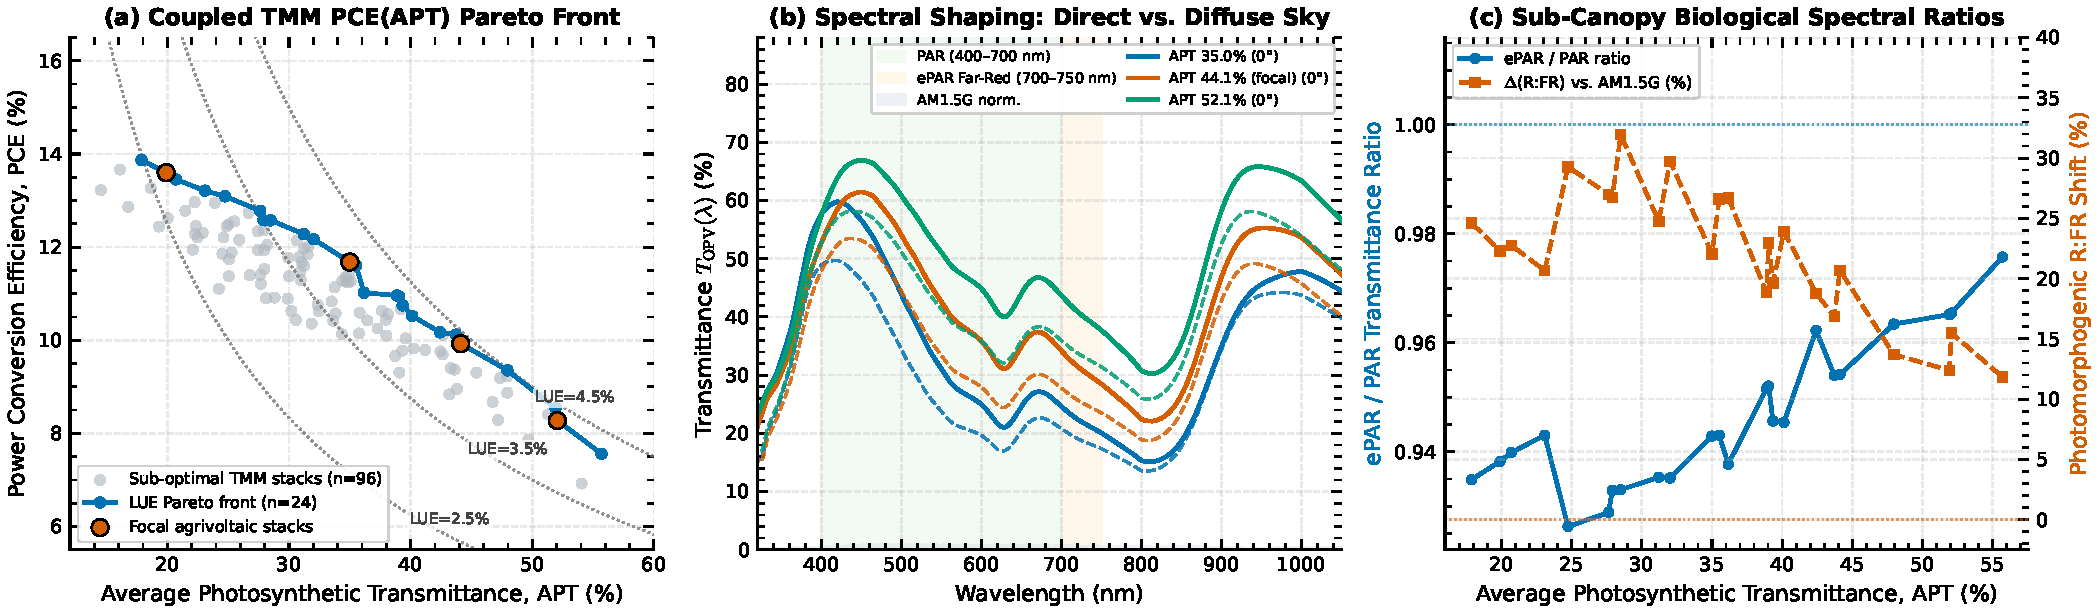
\includegraphics[width=\textwidth]{Fig1_Optical_Pareto_Spectral_TMM.pdf}
 \caption{Transfer-matrix optical design of PM6:Y6 semi-transparent organic photovoltaic (ST-OPV) canopies. (a) Coupled $\mathrm{PCE}(\mathrm{APT})$ Pareto frontier across \num{120} simulated stacks ($n=24$ Pareto optimal, $\mathrm{LUE}_{\max}=\qty{4.424}{\percent}$ in library), highlighting the four focal agrivoltaic designs ($\mathrm{APT}\approx \qty{20}{\percent}$, \qty{35}{\percent}, \qty{44.1}{\percent}, \qty{52.1}{\percent}). (b) Direct normal (\ang{0}, solid) versus diffuse hemispherical (dashed) spectral transmittance across PAR (green shading) and far-red ePAR bands (orange shading). (c) Sub-canopy $\mathrm{ePAR}/\mathrm{PAR}$ ratio and photomorphogenic $\Delta(\mathrm{R{:}FR})$ shift.}
 \label{fig:opt_pareto}
\end{figure}

Sweeping active, metal, and capping thicknesses establishes a sharp $\mathrm{PCE}$--$\mathrm{APT}$ Pareto front bounded between $\mathrm{APT}=\qty{14.54}{\percent}$ and \qty{52.06}{\percent} ($\mathrm{LUE}_{\max}=\qty{4.424}{\percent}$ across the Pareto-optimal subset; \qty{4.486}{\percent} grid peak; \cref{fig:opt_pareto}a); the model reproduces the experimental PM6:Y6 benchmark~\cite{Shen2025NatCommun} on an opaque reference cell to within \qty{5}{\percent} relative ($d_{\mathrm{act}}=\qty{75}{\nano\meter}$, $d_{\mathrm{Ag}}=\qty{100}{\nano\meter}$: $J_{\mathrm{sc}}=\qty{25.70}{\milli\ampere\per\square\centi\meter}$, $\mathrm{PCE}=\qty{15.50}{\percent}$ vs.\ measured \qty{26.36}{\milli\ampere\per\square\centi\meter} and \qty{16.27}{\percent}). Against published semi-transparent PM6:Y6 experimental devices, the Pareto front closely tracks the reported efficiency--transparency trade-off---yielding $\mathrm{PCE}=\qtyrange{13.60}{13.87}{\percent}$ at $\mathrm{APT}=\qtyrange{17.87}{19.90}{\percent}$ versus measured \qty{12.37}{\percent} at \qty{18.6}{\percent} average visible transmittance (AVT)~\cite{Hu2020SciBull}, and $\mathrm{PCE}=\qtyrange{10.75}{10.96}{\percent}$ at $\mathrm{APT}=\qtyrange{38.88}{39.35}{\percent}$ versus measured \qty{10.57}{\percent} at \qty{38.21}{\percent} AVT~\cite{Xue2025AFM}---noting that AVT applies photopic luminosity weighting whereas APT weights photon flux uniformly across \qtyrange{400}{700}{\nano\meter}, and no physical prototype of the focal $\mathrm{APT44}$ stack was fabricated here. Selecting the focal balance stack $\mathrm{APT44}$ ($d_{\mathrm{act}}=\qty{60}{\nano\meter}$, $d_{\mathrm{Ag}}=\qty{12}{\nano\meter}$, $d_{\mathrm{cap}}=\qty{35}{\nano\meter}$) achieves $\mathrm{APT}=\qty{44.12}{\percent}$ and $\mathrm{PCE}=\qty{9.93}{\percent}$ at AM1.5G, whereas thinner silver/active stacks raise transparency to $\mathrm{APT}=\qty{52.1}{\percent}$ ($\mathrm{PCE}\approx \qty{8.3}{\percent}$). Spectral transmittance curves (\cref{fig:opt_pareto}b) show pronounced blue--green transmission (\qtyrange{420}{540}{\nano\meter}, peaking above \qty{61}{\percent} for $\mathrm{APT44}$) paired with strong PM6:Y6 absorption across the red--NIR region (\qtyrange{600}{850}{\nano\meter}). Hemispherical diffuse transmittance sits \numrange{5}{10}~percentage points below \ang{0} normal beam transmittance due to higher oblique Fresnel reflection---a non-negligible penalty during humid Cameroon monsoons where diffuse sky fractions reach \qtyrange{41.6}{50.2}{\percent}. Across Pareto designs, differential attenuation near Y6's \qty{700}{\nano\meter} band edge keeps $\mathrm{ePAR}/\mathrm{PAR} \in [\num{0.926}, \num{0.976}]$ while moderately shifting transmitted $\mathrm{R{:}FR}$ by \qtyrange{+11}{+32}{\percent} (\cref{fig:opt_pareto}c).

\subsection{Microclimatic cooling, seasonal regime inversion, and four-lever attribution}
\label{sec:res_agro}

\begin{figure}[htbp]
 \centering
 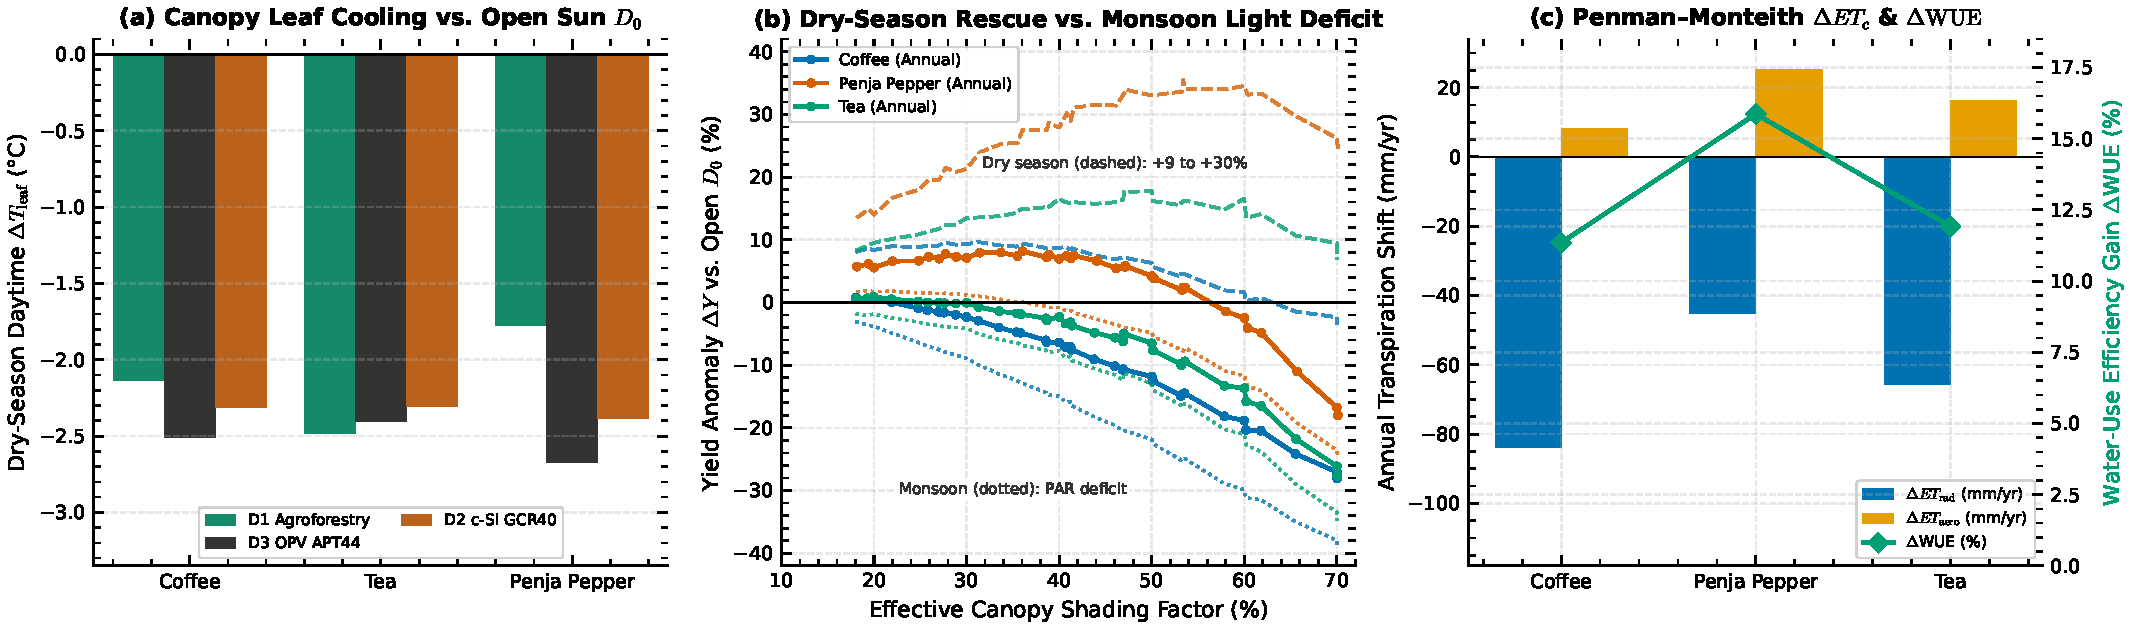
\includegraphics[width=\textwidth]{Fig3_Microclimate_Cooling_Dry_Wet_Regimes.pdf}
 \caption{Hourly ERA5 microclimate and seasonal agronomic divergence across Cameroon highlands. (a) Dry-season daytime leaf cooling ($\Delta T_{\mathrm{leaf}}$) relative to open sun $D_0$ across agroforestry ($D_1$), c-Si ($D_2$), and ST-OPV ($D_3$). (b) Annual (solid), dry-season (dashed), and monsoon wet-season (dotted) assimilation-based yield proxies versus effective canopy shading factor. (c) Penman--Monteith radiative ($\Delta ET_{\mathrm{rad}}$) versus aerodynamic ($\Delta ET_{\mathrm{aero}}$) transpiration shifts and water-use efficiency gains ($\Delta\mathrm{WUE}$) under the focal balanced design $D_3(\mathrm{APT44,\,GCR65})$.}
 \label{fig:microclimate}
\end{figure}

\cref{fig:microclimate} and \cref{tab:agro_summary} show a seasonal sign inversion in the modeled assimilation-based canopy yield proxy across all three crops. During intense dry-season midday heat, partial shading cuts canopy radiative load and cools leaves by \qtyrange{-1.51}{-2.67}{\celsius} rainfed ($\Delta T_{\mathrm{leaf}}$) and by \qtyrange{-3.10}{-3.45}{\celsius} with supplemental irrigation ($D_5$; \cref{fig:microclimate}a). Simultaneously, spectrally selective transmittance lowers daytime module self-heating on $D_3(\mathrm{APT44,\,GCR65})$ to $\Delta T_{\mathrm{PV}} = \qtyrange{3.56}{4.29}{\celsius}$ above ambient versus \qtyrange{7.73}{9.47}{\celsius} on opaque $D_2(\mathrm{c\text{-}Si,\,GCR40})$, curbing NFA efficiency derating relative to c-Si even though both systems produce similar leaf cooling (\qtyrange{-2.40}{-2.67}{\celsius} vs.\ \qtyrange{-2.31}{-2.38}{\celsius}). Because Foumbot ($\mathrm{VPD}_{95} = \qty{4.07}{\kilo\pascal}$) and Njombe-Penja ($T_{\max} = \qty{35.8}{\celsius}$) frequently cross stomatal closure and photoinhibition thresholds ($I_{\mathrm{PI}}=\qtyrange{900}{1100}{\micro\mole\per\square\meter\per\second}$), shading delivers strong dry-season assimilation gains under $D_3(\mathrm{APT44,\,GCR65})$ of \qty{+8.82}{\percent} (coffee), \qty{+15.98}{\percent} (tea), and \qty{+30.24}{\percent} (Penja white pepper; \cref{fig:microclimate}b, dashed curves). Simultaneously, Penman--Monteith transpiration declines (\qtyrange{-7.28}{-16.56}{\percent}) because radiative suppression ($\Delta ET_{\mathrm{rad}} = \qty{-83.98}{\milli\meter\per\yr}$ in coffee, \qty{-65.72}{\milli\meter\per\yr} in tea, and \qty{-45.29}{\milli\meter\per\yr} in pepper) dominates modest rainfed aerodynamic increases ($\Delta ET_{\mathrm{aero}} = \qtylist{+8.22;+16.41;+25.18}{\milli\meter\per\yr}$), lifting crop water-use efficiency ($\Delta\mathrm{WUE}$) by \qty{+11.35}{\percent} in coffee, \qty{+11.92}{\percent} in tea, and \qty{+15.87}{\percent} in Penja white pepper (\cref{fig:microclimate}c); dry-season irrigation in $D_5$ restores stomatal conductance and drives $\Delta ET_{\mathrm{aero}}$ up to \qtyrange{+43.26}{+63.17}{\milli\meter\per\yr}.

However, overcast monsoon conditions invert this mechanism: \qtyrange{36.1}{41.6}{\percent} of daytime hours under $\mathrm{GCR}=\qty{65}{\percent}$ fall into light-limited PAR regimes ($F_{\mathrm{lp}}$), inflicting wet-season assimilation losses of \qty{-15.88}{\percent} in Arabica coffee and \qty{-8.84}{\percent} in highland tea (\cref{fig:microclimate}b, dotted curves). Benchmarked against traditional agroforestry ($D_1$, which achieves annual yield proxies of \qty{-2.35}{\percent} in coffee at \qty{32.5}{\percent} shade, \qty{+7.96}{\percent} in pepper at \qty{27.5}{\percent} shade, and \qty{-1.81}{\percent} in tea at \qty{40.0}{\percent} shade), rainfed coffee under $D_3(\mathrm{APT44,\,GCR65})$ drops \qty{-7.08}{\percent} annually and tea drops \qty{-3.35}{\percent} (near neutral at \qty{-1.21}{\percent} and \qty{+0.01}{\percent} only at sparse $D_3(\mathrm{APT56,\,GCR50})$), whereas in 2023 PGI Penja white pepper sustains net annual gains of \qty{+7.27}{\percent} under $D_3(\mathrm{APT56,\,GCR50})$, \qty{+8.16}{\percent} under $D_3(\mathrm{APT52,\,GCR65})$, and \qty{+7.43}{\percent} under $D_3(\mathrm{APT44,\,GCR65})$ (\cref{tab:agro_summary}). Across 2014--2023 ERA5 forcing, however, pepper yields remain positive in only seven of ten years (decade median \qty{+2.99}{\percent}, mean \qty{+2.73}{\percent}, range \qtyrange{-1.43}{+7.60}{\percent}), whereas coffee (\qty{-8.25}{\percent} median, \qtyrange{-11.45}{-7.08}{\percent}) and tea (\qty{-3.36}{\percent} median, \qtyrange{-5.85}{-1.86}{\percent}) stay negative in all ten years (\cref{sec:weather_year_sensitivity}; \cref{sm:tab:weather_decade}). Heavy shading (\qty{70}{\percent} effective shade, $D_2(\mathrm{c\text{-}Si,\,GCR70})$ or $D_3(\mathrm{APT20,\,GCR85})$) imposes severe \qtyrange{-16.8}{-28.1}{\percent} penalties across every species, while supplemental irrigation in $D_5$ rescues coffee (\qty{+0.22}{\percent}), lifts tea (\qty{+2.47}{\percent}), and raises 2023 pepper to \qty{+12.25}{\percent}.

\begin{figure}[htbp]
 \centering
 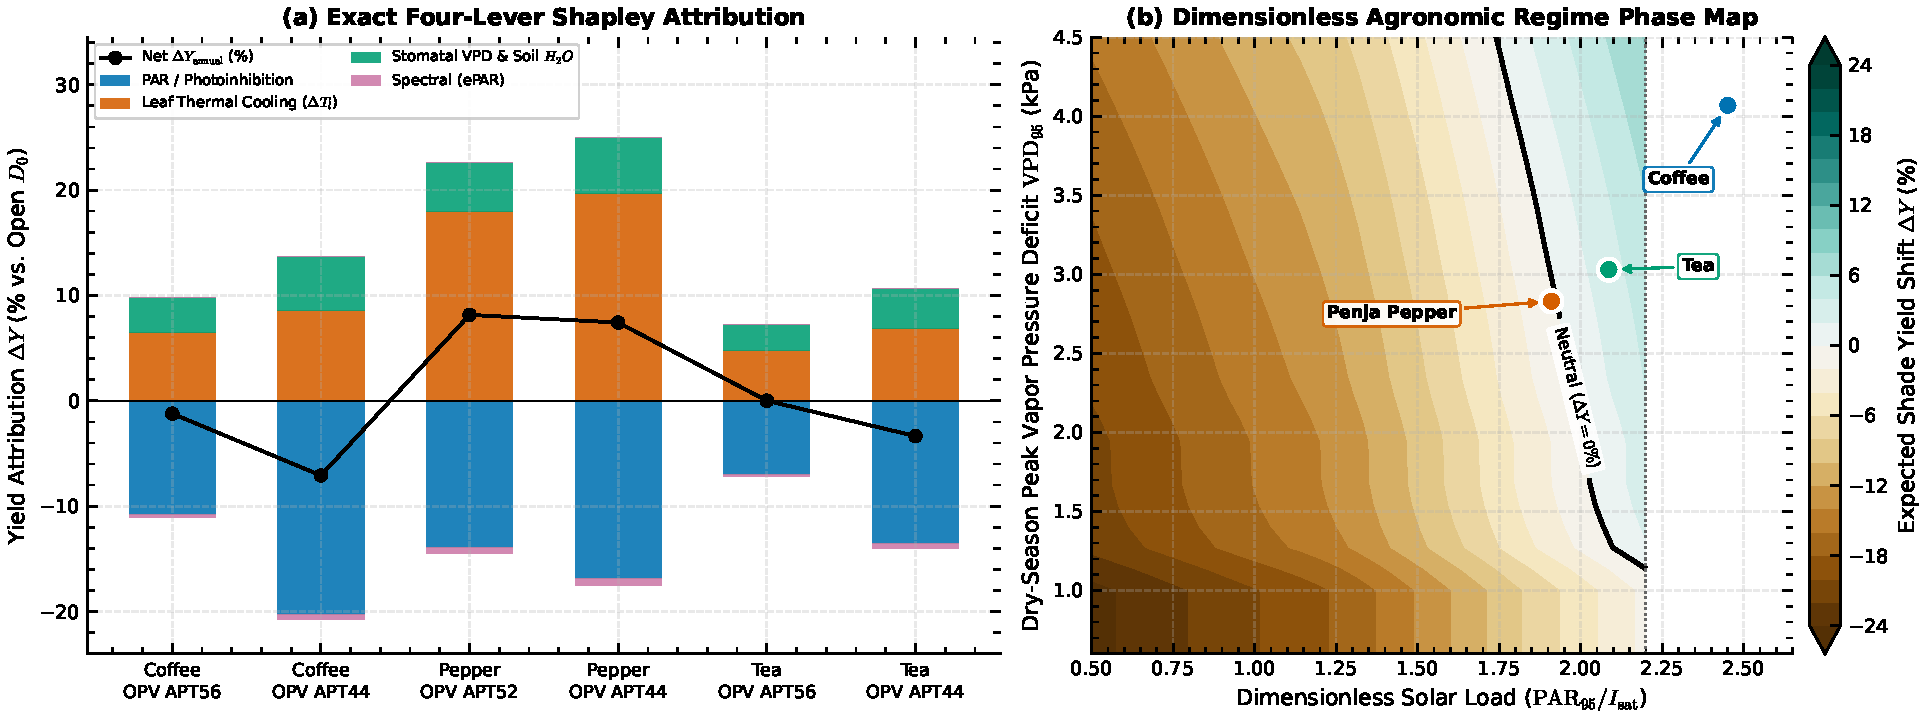
\includegraphics[width=\textwidth]{Fig4_Four_Lever_Causal_Attribution_Phase.pdf}
 \caption{Mechanism attribution and climate-envelope mapping. (a) Exact 16-coalition Shapley attribution partitioning annual assimilation shift $\Delta Y$ (black line) into PAR/photoinhibition, thermal leaf cooling, VPD/soil-water conservation, and spectral ($\mathrm{ePAR}$) levers (residual $\le \qty{7.1e-15}{\percent}$). (b) Agronomic phase diagram in normalized dry-season solar load ($\mathrm{PAR}_{95}/I_{\mathrm{sat}}$) and $\mathrm{VPD}_{95}$, locating the three crops near or above the neutral shade-benefit threshold.}
 \label{fig:shapley}
\end{figure}

Exact four-lever Shapley attribution (\cref{fig:shapley}a) apportions these modeled responses across physical pathways. For Penja white pepper under $D_3(\mathrm{APT52,\,GCR65})$ (\qty{+8.16}{\percent}), thermal leaf cooling (\qty{+17.99}{\percent}) and stomatal/soil moisture conservation (\qty{+4.64}{\percent}) outweigh the PAR reduction penalty (\qty{-13.93}{\percent}), while optical spectral quality ($\phi_{\mathrm{spec+Q}} = \qty{-0.55}{\percent}$) plays a minor sub-percent role. Conversely, in Foumbot coffee under $D_3(\mathrm{APT44,\,GCR65})$ (\qty{-7.08}{\percent}), the PAR penalty (\qty{-20.31}{\percent}) dominates combined thermal (\qty{+8.58}{\percent}) and soil-water (\qty{+5.11}{\percent}) gains. Comparing ST-OPV and elevated c-Si at matched $\sim\qty{40}{\percent}$ shade ($D_3(\mathrm{APT44,\,GCR65})$ vs.\ $D_2(\mathrm{c\text{-}Si,\,GCR40})$; \cref{tab:agro_summary}) reveals nearly indistinguishable annual crop responses---differing by at most \qty{1.05}{pp} (\qty{-7.08}{\percent} vs.\ \qty{-6.38}{\percent} in coffee, \qty{+7.43}{\percent} vs.\ \qty{+6.95}{\percent} in pepper, \qty{-3.35}{\percent} vs.\ \qty{-2.30}{\percent} in tea). Across ST-OPV designs ($\mathrm{APT56}$--$\mathrm{APT44}$), $\phi_{\mathrm{spec+Q}}$ stays within \qtyrange{-0.21}{-0.67}{\percent} because PM6:Y6 band-edge absorption trims transmitted $\mathrm{ePAR}/\mathrm{PAR}$ below sunlight; isolating $\eta_{\mathrm{NESS}}\equiv 1$ shows classical spectral weighting explains essentially the entire term ($\phi_{\mathrm{spec}} = \qtylist{-0.477;-0.668;-0.516}{\percent}$), with marginal CW quantum contribution $|\phi_{\mathrm{spec+Q}}-\phi_{\mathrm{spec}}| \le \qty{4.3e-4}{pp}$. Including bounded photomorphogenic plasticity ($V_{c\max 25}, J_{\max 25}$ modulated by \qtyrange{-2}{+5}{\percent} under the \qty{+5.99}{\percent} elevated sub-canopy $\mathrm{R{:}FR}$) spans \qtyrange{-8.70}{-3.17}{\percent} (coffee), \qtyrange{+4.92}{+13.58}{\percent} (pepper), and \qtyrange{-4.99}{+0.66}{\percent} (tea), confirming sensitivity to unmodeled spectral acclimation (\cref{sm:sec:sm_extensions}). Crucially, the matched-shade comparison equalizes crop light rather than electrical service: $D_3(\mathrm{APT44,\,GCR65})$ generates only \qtyrange{81.0}{83.0}{\percent} of $D_2(\mathrm{c\text{-}Si,\,GCR40})$ power in 2023 (\qtyrange{81.2}{82.8}{\percent} over 2014--2023). Solving instead for exact energy-matched c-Si ($D_{2,\mathrm{EM}}$, $\mathrm{GCR}=\qtyrange{32.4}{33.2}{\percent}$) delivers \qtyrange{2.9}{3.6}{pp} stronger yields in coffee (\qty{-3.44}{\percent}) and tea (\qty{-0.44}{\percent}), virtually equal pepper yield (\qty{+7.29}{\percent}), and \qtyrange{268}{328}{\kUSD\per\hectare} higher NPV than $D_3$ (\cref{sm:sec:sm_extensions}). Mapping peak irradiance normalized by species saturation ($I_{\mathrm{sat}}$) against $\mathrm{VPD}_{95}$ (\cref{fig:shapley}b) summarizes the rainfed climate envelope.

\begin{table}[htbp]
 \centering
 \caption{Focal seasonal assimilation-based yield proxies, exact four-lever Shapley decomposition ($\phi_i$), water-use shift ($\Delta\mathrm{WUE}$), and annual PV yield across Cameroon perennials.}
 \label{tab:agro_summary}
 \scriptsize
 \resizebox{\textwidth}{!}{
\begin{tabular}{@{}llrrrrrrrrr@{}}
 \toprule
 \textbf{Crop} & \textbf{Scenario} & \textbf{Shade} & $\Delta Y_{\mathrm{ann}}$ & $\Delta Y_{\mathrm{dry}}$ & $\Delta Y_{\mathrm{wet}}$ & $\phi_{\mathrm{PAR/PI}}$ & $\phi_{\mathrm{therm}}$ & $\phi_{\mathrm{H_2O}}$ & $\Delta\mathrm{WUE}$ & \textbf{PV} \\
 & & (\unit{\percent}) & (\unit{\percent}) & (\unit{\percent}) & (\unit{\percent}) & (\unit{\percent}) & (\unit{\percent}) & (\unit{\percent}) & (\unit{\percent}) & (\unit{\MWh\per\hectare}) \\
 \midrule
 Coffee & $D_3$ (APT56, GCR50) & \num{25.7} & \num{-1.21} & \num{+9.02} & \num{-6.96} & \num{-10.82} & \num{+6.45} & \num{+3.37} & \num{+7.80} & \num{717.0} \\
 Coffee & $D_3$ (APT44, GCR65) & \num{40.6} & \num{-7.08} & \num{+8.82} & \num{-15.88} & \num{-20.31} & \num{+8.58} & \num{+5.11} & \num{+11.35} & \num{1223.3} \\
 Coffee & $D_5$ (APT44, GCR65, irrig.) & \num{40.6} & \num{+0.22} & \num{+38.23} & \num{-15.88} & \num{-21.38} & \num{+10.81} & \num{+11.25} & \num{+0.15} & \num{1223.3} \\
 Coffee & $D_2$ (c-Si, GCR40) & \num{40.0} & \num{-6.38} & \num{+8.73} & \num{-14.92} & \num{-19.24} & \num{+8.14} & \num{+4.71} & \num{+9.56} & \num{1479.0} \\
 \midrule
 Pepper & $D_3$ (APT56, GCR50) & \num{25.9} & \num{+7.27} & \num{+19.57} & \num{+1.53} & \num{-8.73} & \num{+13.25} & \num{+3.02} & \num{+11.19} & \num{611.7} \\
 Pepper & $D_3$ (APT52, GCR65) & \num{36.0} & \num{+8.16} & \num{+27.56} & \num{+0.04} & \num{-13.93} & \num{+17.99} & \num{+4.64} & \num{+15.19} & \num{870.2} \\
 Pepper & $D_3$ (APT44, GCR65) & \num{40.8} & \num{+7.43} & \num{+30.24} & \num{-1.36} & \num{-16.87} & \num{+19.69} & \num{+5.27} & \num{+15.87} & \num{1043.7} \\
 Pepper & $D_5$ (APT44, GCR65, irrig.) & \num{40.8} & \num{+12.25} & \num{+49.68} & \num{-1.36} & \num{-17.06} & \num{+21.56} & \num{+8.40} & \num{+9.02} & \num{1043.7} \\
 Pepper & $D_2$ (c-Si, GCR40) & \num{40.0} & \num{+6.95} & \num{+27.89} & \num{-0.78} & \num{-15.72} & \num{+17.90} & \num{+4.75} & \num{+12.11} & \num{1257.2} \\
 \midrule
 Tea & $D_3$ (APT56, GCR50) & \num{25.8} & \num{+0.01} & \num{+11.26} & \num{-3.47} & \num{-6.99} & \num{+4.73} & \num{+2.48} & \num{+8.29} & \num{652.5} \\
 Tea & $D_3$ (APT44, GCR65) & \num{40.7} & \num{-3.35} & \num{+15.98} & \num{-8.84} & \num{-13.53} & \num{+6.84} & \num{+3.86} & \num{+11.92} & \num{1113.3} \\
 Tea & $D_5$ (APT44, GCR65, irrig.) & \num{40.7} & \num{+2.47} & \num{+41.38} & \num{-8.84} & \num{-13.90} & \num{+8.36} & \num{+8.50} & \num{+0.74} & \num{1113.3} \\
 Tea & $D_2$ (c-Si, GCR40) & \num{40.0} & \num{-2.30} & \num{+16.56} & \num{-7.65} & \num{-12.63} & \num{+6.65} & \num{+3.68} & \num{+10.77} & \num{1374.4} \\
 \bottomrule
 \end{tabular}
}
\end{table}

\subsection{Cooperative dispatch, dual-FU LCA, and break-even frontiers}
\label{sec:res_tea}

\begin{figure}[htbp]
 \centering
 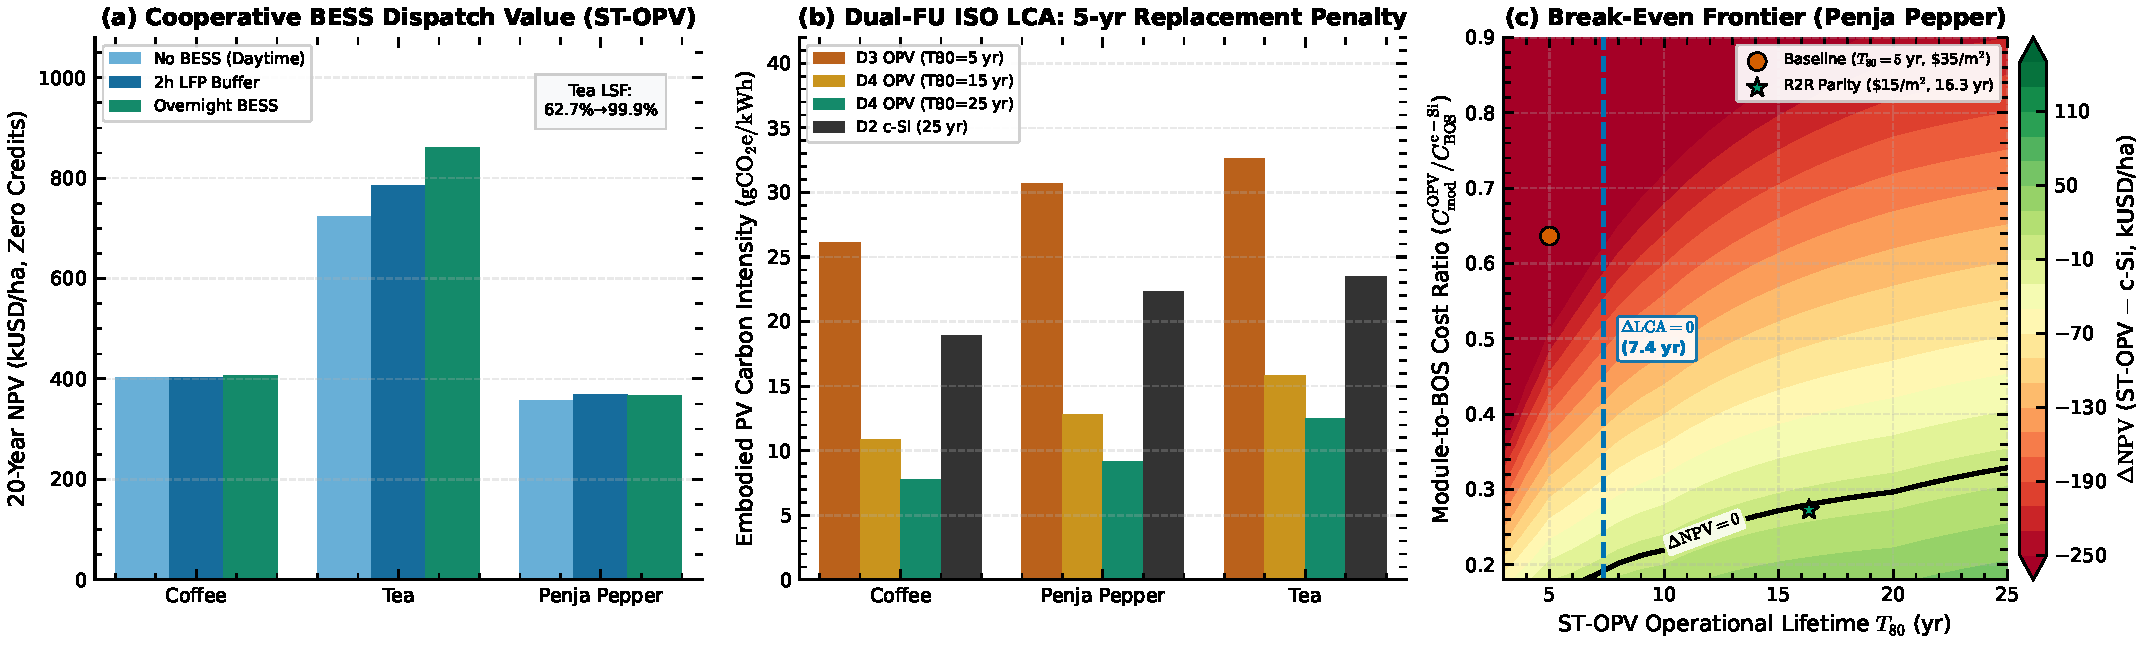
\includegraphics[width=\textwidth]{Fig5_Dispatch_TEA_LCA_BreakEven.pdf}
 \caption{Techno-economic dispatch, environmental carbon intensity, and parity thresholds (\qty{0}{\USD\per\tCOtwoe}, \qty{0}{\percent} subsidy baseline). (a) Effect of battery dispatch on \qty{20}{\yr} NPV for $D_3(\mathrm{APT44,\,GCR65})$ across daytime-only operation, a \qty{2}{\hour} LFP buffer, and an overnight-withering LFP system, highlighting Djuttitsa tea load solar fraction ($\mathrm{LSF}$) climbing from \qty{62.7}{\percent} to \qty{99.9}{\percent}. (b) Embodied PV carbon intensity across \qty{5}{\yr} ($D_3$), \qty{15}{\yr} / \qty{25}{\yr} encapsulated ST-OPV ($D_4$), and \qty{25}{\yr} c-Si ($D_2$). (c) Two-dimensional NPV and LCA parity frontier over ST-OPV operational lifetime ($T_{80}\ge\qty{1}{\yr}$) and module-to-BOS cost ratio for Penja white pepper, with c-Si BOS sampled over \qtyrange{35}{85}{\USD\per\square\meter}.}
 \label{fig:tea_lca}
\end{figure}

Integrating cooperative processing dispatch sharply separates Djuttitsa tea from daytime-dominated coffee and pepper cooperatives (\cref{fig:tea_lca}a, \cref{tab:tea_lca}). Because tea withering consumes \qty{45}{\percent} of its \qty{307.8}{\MWh\per\yr} factory electricity overnight, shifting from daytime-only dispatch to overnight LFP storage raises load solar fraction from \qty{62.68}{\percent} to \qty{99.92}{\percent} and lifts \qty{20}{\yr} NPV from \qty{724.1}{\kUSD\per\hectare} ($\mathrm{IRR} = \qty{38.65}{\percent}$) to \qty{860.8}{\kUSD\per\hectare} ($\mathrm{IRR} = \qty{35.52}{\percent}$, discounted payback period $\mathrm{DPBP} = \qty{3.01}{\yr}$, $\mathrm{LCOE} = \qty{0.0886}{\USD\per\kWh}$), delivering \qty{393.2}{\tCOtwoe\per\hectare\per\yr} in net areal abatement (\qty{427.3}{\tCOtwoe\per\hectare\per\yr} gross). By contrast, daytime coffee and pepper loads already achieve $\mathrm{LSF} = \qtyrange{88.6}{92.4}{\percent}$ without storage, gaining little from overnight BESS (\qty{403.5}{\kUSD\per\hectare} coffee, \qty{368.4}{\kUSD\per\hectare} pepper with \qty{2}{\hour} buffer). Benchmark ground-mounted PV-only ($D_{\mathrm{PV}}$, c-Si $\mathrm{GCR}=\qty{70}{\percent}$, zero crop revenue) attains \qtyrange{1114.4}{1946.7}{\kUSD\per\hectare} across $C_{\mathrm{BOS}}^{\mathrm{ground}}=\qtyrange{15}{35}{\USD\per\square\meter}$, exceeding elevated $D_2$ agrivoltaic NPV whenever $C_{\mathrm{BOS}}^{\mathrm{ground}} \le \qtyrange{86.4}{108.9}{\USD\per\square\meter}$ (\cref{sm:sec:sm_extensions}).

Under dual-FU ISO~14040/14044 LCA ($T_{80}=\qty{5}{\yr}$ baseline; \cref{fig:tea_lca}b), frequent ST-OPV replacement raises embodied intensity (\qtyrange{26.2}{32.7}{\gCOtwoe\per\kWh}) above \qty{25}{\yr} c-Si (\qtyrange{18.9}{23.5}{\gCOtwoe\per\kWh}). Environmental parity occurs at $T_{80,\mathrm{LCA}}^* = \qty{7.42}{\yr}$ (coffee), \qty{7.40}{\yr} (pepper), and \qty{8.12}{\yr} (tea); under $D_4$ encapsulation ($T_{80}=\qtyrange{15}{25}{\yr}$), ST-OPV intensity falls to \qtyrange{10.8}{15.9}{\gCOtwoe\per\kWh} (\qty{15}{\yr}) and \qtyrange{7.8}{12.5}{\gCOtwoe\per\kWh} (\qty{25}{\yr}), tightening LCOE to \qtylist{0.0422;0.0497;0.0646}{\USD\per\kWh}. Economic parity is far stricter (\cref{fig:tea_lca}c): at \qty{35}{\USD\per\square\meter} modules, ST-OPV never reaches financial parity with c-Si across the tested horizon because elevated c-Si generates \qtyrange{21}{24}{\percent} more electricity per hectare. Only once roll-to-roll manufacturing compresses module CAPEX to \qty{15}{\USD\per\square\meter} ($C_{\mathrm{mod}}^{\mathrm{OPV}} / C_{\mathrm{BOS}}^{\mathrm{c\text{-}Si}} = \num{0.273}$) does NPV parity emerge at $T_{80,\mathrm{NPV}}^* = \qty{16.33}{\yr}$ for Penja white pepper; coffee and tea remain unachievable within both the \qty{20}{\yr} evaluation horizon and the \qty{25}{\yr} tested range. Crediting $\mathrm{kW}$-scaled inverter/interconnection charges (\qtyrange{100}{200}{\USD\per\kWp}) narrows ST-OPV's $\Delta\mathrm{NPV}$ deficit by only \qtyrange{24.2}{48.4}{\kUSD\per\hectare} ($<\qty{15}{\percent}$ of the baseline gap; \cref{sm:sec:sm_extensions}).

\begin{table}[htbp]
 \centering
 \caption{Techno-economic and life-cycle comparison ($D_3(\mathrm{APT44,\,GCR65})$ vs.\ $D_2(\mathrm{c\text{-}Si,\,GCR40})$) and break-even thresholds at the strict zero-subsidy baseline (\qty{0}{\USD\per\tCOtwoe}, $\mathrm{WACC} = \qty{10}{\percent}$).}
 \label{tab:tea_lca}
 \scriptsize
 \resizebox{\textwidth}{!}{
\begin{tabular}{@{}llrrrrrrr@{}}
 \toprule
 \textbf{Crop} & \textbf{System / Dispatch} & \textbf{LSF} & \textbf{LER} & \textbf{NPV} & \textbf{IRR} & \textbf{LCOE} & \textbf{LCA} & \textbf{Off-Grid NPV} \\
 & & (\unit{\percent}) & (--) & (\unit{\kUSD\per\hectare}) & (\unit{\percent}) & (\unit{\USD\per\kWh}) & (\unit{\gCOtwoe\per\kWh}) & (\unit{\kUSD\per\hectare}) \\
 \midrule
 Coffee & ST-OPV (no BESS) & \num{92.42} & \num{1.401} & \num{402.5} & \num{26.46} & \num{0.0625} & \num{25.90} & -- \\
 Coffee & ST-OPV (\qty{2}{\hour} BESS) & \num{100.00} & \num{1.401} & \num{403.5} & \num{26.16} & \num{0.0637} & \num{26.16} & \num{-379.8} \\
 Coffee & c-Si (\qty{2}{\hour} BESS) & \num{100.00} & \num{1.507} & \num{779.3} & \num{34.77} & \num{0.0380} & \num{18.92} & -- \\
 \midrule
 Penja Pepper & ST-OPV (no BESS) & \num{88.62} & \num{1.548} & \num{358.0} & \num{24.72} & \num{0.0733} & \num{30.36} & -- \\
 Penja Pepper & ST-OPV (\qty{2}{\hour} BESS) & \num{99.97} & \num{1.548} & \num{368.4} & \num{24.74} & \num{0.0750} & \num{30.73} & \num{-281.5} \\
 Penja Pepper & c-Si (\qty{2}{\hour} BESS) & \num{99.99} & \num{1.640} & \num{709.1} & \num{32.55} & \num{0.0449} & \num{22.31} & -- \\
 \midrule
 Highland Tea & ST-OPV (no BESS) & \num{62.68} & \num{1.429} & \num{724.1} & \num{38.65} & \num{0.0687} & \num{28.46} & -- \\
 Highland Tea & ST-OPV (\qty{2}{\hour} BESS) & \num{74.30} & \num{1.429} & \num{785.7} & \num{39.02} & \num{0.0727} & \num{29.32} & -- \\
 Highland Tea & ST-OPV (overnight BESS) & \num{99.92} & \num{1.429} & \num{860.8} & \num{35.52} & \num{0.0886} & \num{32.66} & \num{+319.8} \\
 Highland Tea & c-Si (overnight BESS) & \num{100.00} & \num{1.548} & \num{1272.6} & \num{41.66} & \num{0.0555} & \num{23.46} & -- \\
 \bottomrule
 \end{tabular}
}
\end{table}

\subsection{Sobol uncertainty quantification and policy stress tests}
\label{sec:res_sobol}

\begin{figure}[htbp]
 \centering
 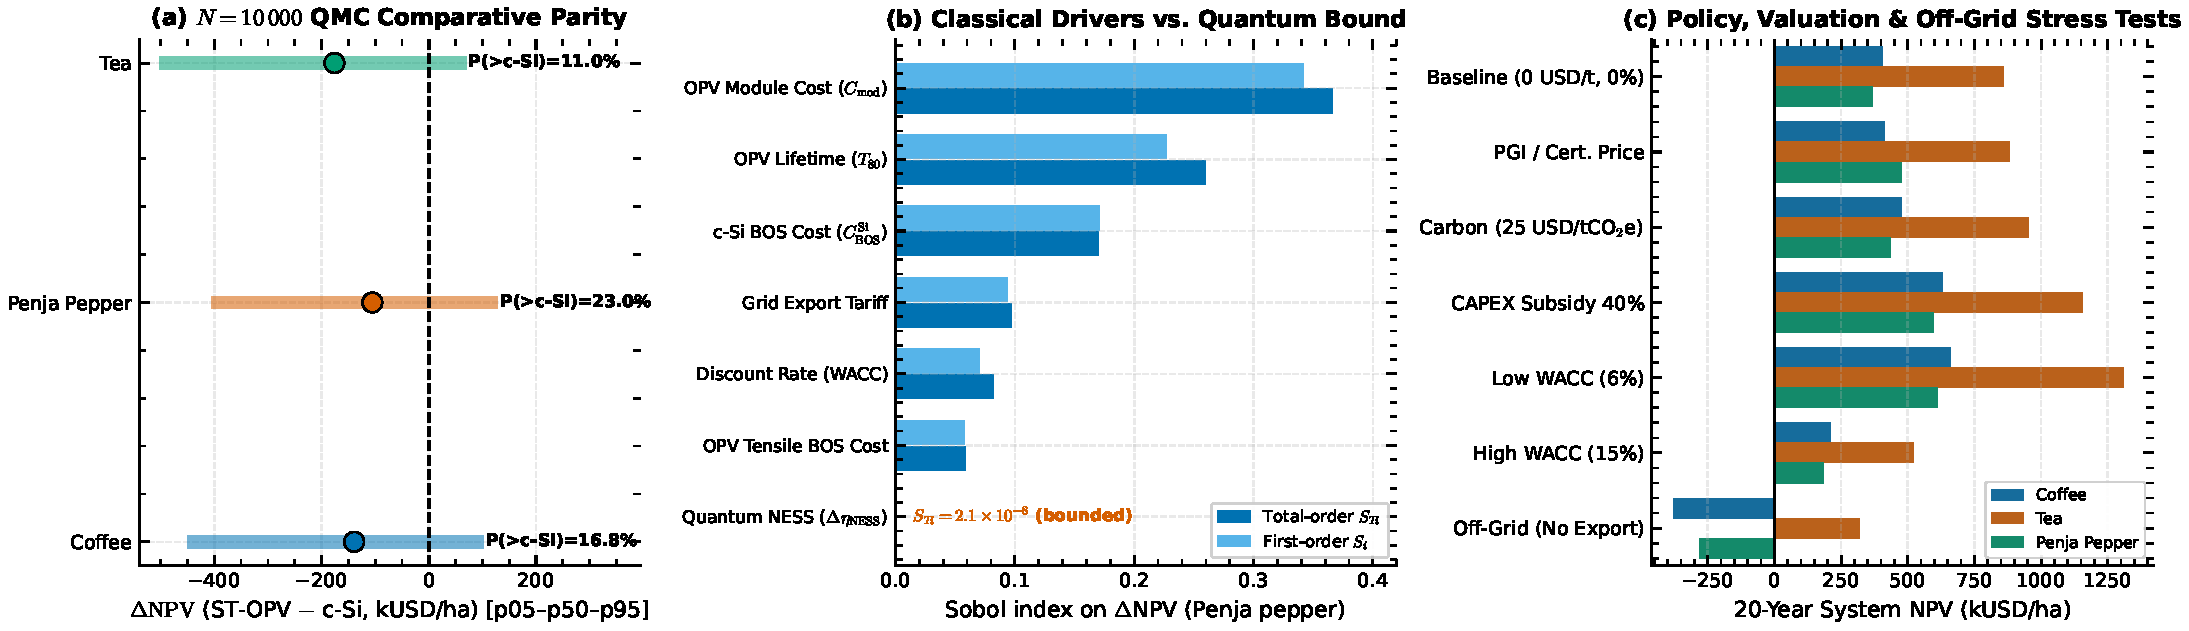
\includegraphics[width=\textwidth]{Fig6_Sobol_Uncertainty_LER_Policy.pdf}
 \caption{Probabilistic parity and global variance attribution ($N = \num{10000}$ Saltelli QMC draws). (a) Comparative $\Delta\mathrm{NPV} = \mathrm{NPV}_{\mathrm{OPV}} - \mathrm{NPV}_{\mathrm{Si}}$ [p05--p50--p95] distributions and exceedance probabilities. (b) Ranked first-order ($S_i$) and total-order ($S_{Ti}$) Sobol indices on Penja white pepper $\Delta\mathrm{NPV}$ alongside the bounded quantum NESS index ($S_{Ti} = \num{2.10e-8}$; $\le \num{2.58e-7}$ under the exact-HEOM envelope). (c) Policy, valuation, discount-rate, and off-grid stress tests across the three crops ($D_3(\mathrm{APT44,\,GCR65})$).}
 \label{fig:sobol}
\end{figure}

Across $N=\num{10000}$ Saltelli quasi-Monte Carlo parameter realizations spanning the full 12-parameter uncertainty box (carbon pricing $[\num{0}, \num{25}]\,\unit{\USD\per\tCOtwoe}$; \cref{fig:sobol}a), ST-OPV exceeds elevated c-Si NPV in only \qty{23.0}{\percent} of Penja white pepper draws (median \qty{-105.3}{\kUSD\per\hectare}, p05--p95 \qtyrange{-394.4}{+116.9}{\kUSD\per\hectare}), \qty{16.8}{\percent} of Arabica coffee draws (median \qty{-139.3}{\kUSD\per\hectare}, \qtyrange{-437.6}{+90.2}{\kUSD\per\hectare}), and \qty{11.0}{\percent} of tea draws (median \qty{-176.0}{\kUSD\per\hectare}, \qtyrange{-490.0}{+58.0}{\kUSD\per\hectare}), meaning elevated c-Si dominates in \qtyrange{77.0}{89.0}{\percent} of draws. Under strict zero-carbon pricing, ST-OPV exceedance rises only slightly (\qty{24.7}{\percent} pepper, \qty{18.5}{\percent} coffee, \qty{12.3}{\percent} tea; $S_{Ti} \le \num{0.0011}$ on $\Delta\mathrm{NPV}$ vs.\ $\le \num{0.0052}$ on $\mathrm{NPV}_{\mathrm{OPV}}$).

Contrasting Saltelli--Sobol total-order indices between standalone ST-OPV profitability ($\mathrm{NPV}_{\mathrm{OPV}}$) and comparative parity ($\Delta\mathrm{NPV}$) exposes a clear dual-index split (\cref{tab:sobol_dual}, \cref{fig:sobol}b). Standalone ST-OPV installations remain positive across QMC realizations, governed in daytime-dominated coffee and pepper by grid export tariff ($S_{Ti}=\num{0.52}$ and \num{0.43}) and WACC (\num{0.29} and \num{0.32}), whereas energy-intensive tea shifts sensitivity to WACC (\num{0.45}) and avoided diesel price (\num{0.28}). Evaluating technology choice ($\Delta\mathrm{NPV}$) cancels shared macro-financial terms and concentrates $>\qty{74}{\percent}$ of variance on three hardware parameters: OPV module CAPEX ($S_{Ti}=\numrange{0.323}{0.366}$), ST-OPV $T_{80}$ lifetime (\numrange{0.247}{0.267}), and c-Si steel BOS (\numrange{0.150}{0.170}), unchanged across resolution ladders and three QMC scrambles (\cref{sm:tab:sobol_convergence}).

\begin{table}[htbp]
 \centering
 \caption{Dual Saltelli--Sobol decomposition ($N=\num{10000}$ base samples, \num{140000} evaluations per crop) contrasting macro-financial drivers of standalone bankability ($\mathrm{NPV}_{\mathrm{OPV}}$) against hardware engineering drivers of comparative parity ($\Delta\mathrm{NPV} = \mathrm{NPV}_{\mathrm{OPV}} - \mathrm{NPV}_{\mathrm{Si}}$).}
 \label{tab:sobol_dual}
 \scriptsize
 \resizebox{\textwidth}{!}{
 \begin{tabular}{@{}lclrrlc@{}}
 \toprule
 \textbf{Crop} & $\mathrm{NPV}_{\mathrm{OPV}}^{p50}$ $[p05, p95]$ & \textbf{Top $S_{Ti}(\mathrm{NPV}_{\mathrm{OPV}})$ drivers} & $P(\Delta>0)$ & $\Delta\mathrm{NPV}_{p50}$ & \textbf{Top $S_{Ti}(\Delta\mathrm{NPV})$ drivers} & $S_{Ti}^Q$ ($\mathrm{NPV}_{\mathrm{OPV}}$ / $\Delta\mathrm{NPV}$) \\
 & (\unit{\kUSD\per\hectare}) & (parameter, index) & (\unit{\percent}) & (\unit{\kUSD\per\hectare}) & (parameter, index) & (--) \\
 \midrule
 Arabica coffee & \num{562.3} [\num{145.0}, \num{1116.5}] & Tariff (\num{0.518}), WACC (\num{0.287}), $C_{\mathrm{mod}}^{\mathrm{OPV}}$ (\num{0.104}) & \num{16.75} & \num{-139.3} & $C_{\mathrm{mod}}^{\mathrm{OPV}}$ (\num{0.343}), $T_{80}$ (\num{0.247}), $C_{\mathrm{BOS}}^{\mathrm{c\text{-}Si}}$ (\num{0.159}) & \num{1.16e-9} / \num{3.83e-9} \\
 Penja white pepper & \num{537.8} [\num{148.4}, \num{1038.5}] & Tariff (\num{0.426}), WACC (\num{0.320}), $C_{\mathrm{mod}}^{\mathrm{OPV}}$ (\num{0.125}) & \num{22.99} & \num{-105.3} & $C_{\mathrm{mod}}^{\mathrm{OPV}}$ (\num{0.366}), $T_{80}$ (\num{0.260}), $C_{\mathrm{BOS}}^{\mathrm{c\text{-}Si}}$ (\num{0.170}) & \num{7.15e-9} / \num{2.10e-8} \\
 Highland tea & \num{1042.8} [\num{505.6}, \num{1780.2}] & WACC (\num{0.450}), Diesel (\num{0.282}), Tariff (\num{0.147}) & \num{11.00} & \num{-176.0} & $C_{\mathrm{mod}}^{\mathrm{OPV}}$ (\num{0.323}), $T_{80}$ (\num{0.267}), $C_{\mathrm{BOS}}^{\mathrm{c\text{-}Si}}$ (\num{0.150}) & \num{1.89e-9} / \num{9.85e-9} \\
 \bottomrule
 \end{tabular}
 }
\end{table}

Policy stress tests (\cref{fig:sobol}c) highlight export dependence: removing export on an export-sized array cuts NPV to \qty{-379.8}{\kUSD\per\hectare} (coffee) and \qty{-281.5}{\kUSD\per\hectare} (pepper), whereas tea retains \qty{+319.8}{\kUSD\per\hectare} ($\mathrm{IRR} = \qty{20.1}{\percent}$, $\mathrm{DPBP}=\qty{6.6}{\yr}$). When off-grid arrays are instead scaled down to match local demand ($\alpha = \qty{0.07}{\hectare}$ coffee, \qty{0.08}{\hectare} pepper, \qty{0.39}{\hectare} tea), net parcel NPV turns strongly positive (\qtylist{+188.7;+227.4;+665.4}{\kUSD\per\hectare}, \qtyrange{+160.3}{+622.8}{\kUSD\per\hectare} over $D_0$; \cref{sm:sec:sm_extensions}). PGI Penja pricing (\qty{14000}{\XAF\per\kilogram}) adds $\sim\qty{100}{\kUSD\per\hectare}$, while concessional finance ($\mathrm{WACC} = \qty{6}{\percent}$) matches a \qty{40}{\percent} upfront CAPEX grant.

% ==============================================================================
\section{Quantum-to-system boundary analysis: pulsed coherent dynamics vs.\ CW sunlight}
\label{sec:quantum_bound}
% ==============================================================================

\begin{figure}[htbp]
 \centering
 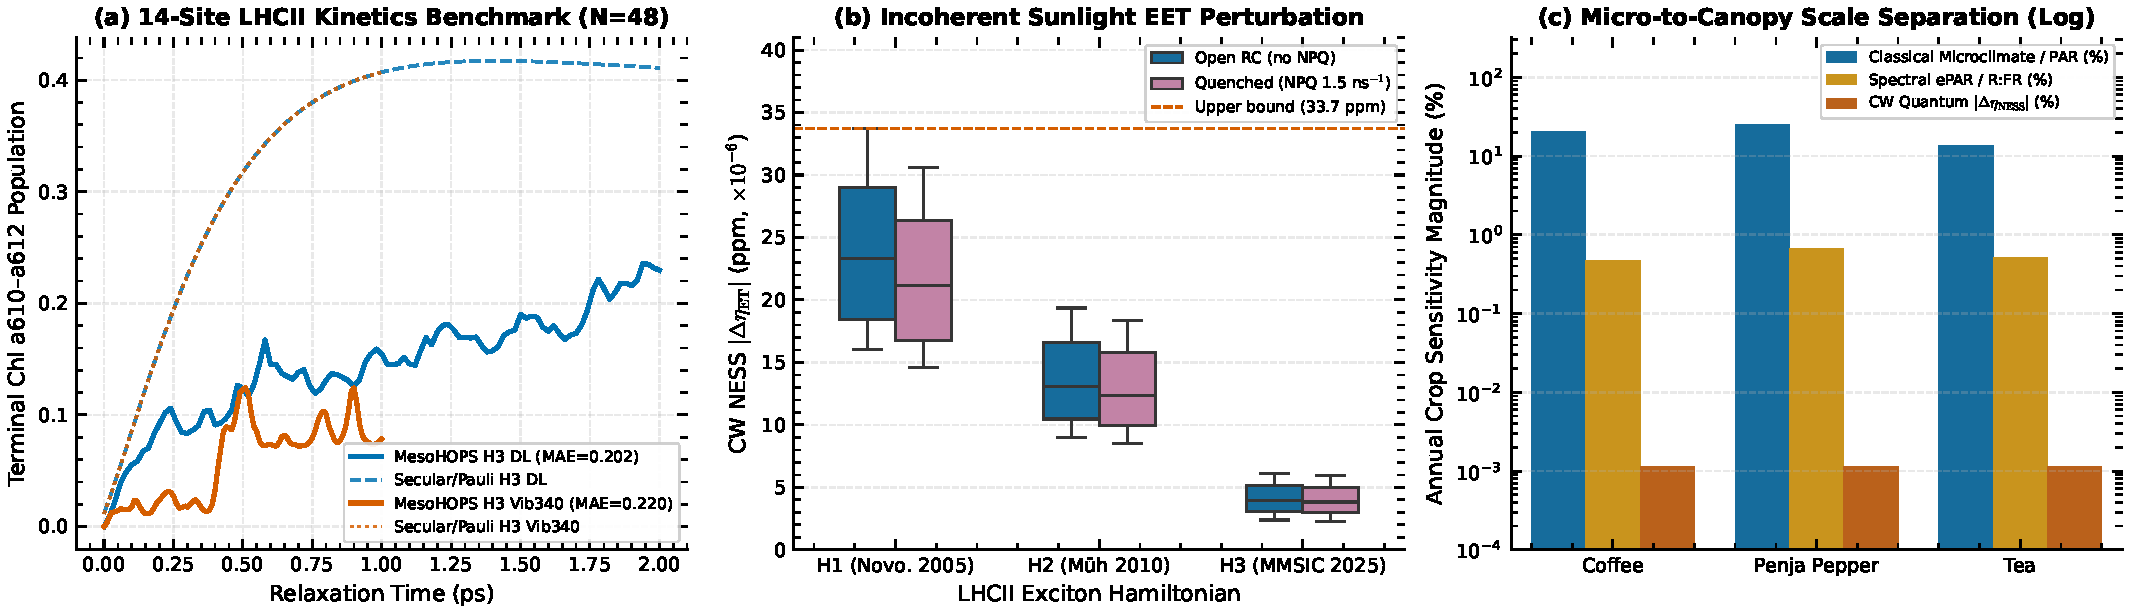
\includegraphics[width=\textwidth]{Fig2_Quantum_NESS_Bound_Benchmark.pdf}
 \caption{Microscopic open-quantum light-harvesting validation and canopy scale separation. (a) Full non-Markovian 14-site MesoHOPS~1.8.0 pulsed excitation kinetics ($N = 48$ disorder draws, $T=\qty{295}{\kelvin}$) versus diagonal secular Pauli kinetics on H3 (Drude--Lorentz bath alone to \qty{2.0}{\pico\second} and augmented with the \qty{340}{\per\centi\meter} vibronic mode to \qty{1.0}{\pico\second}). (b) Continuous-wave (CW) solar NESS perturbation $|\Delta\eta_{\mathrm{ET}}|$ across ST-OPV transmittance spectra (\ang{0} beam and diffuse) and three independent LHCII Hamiltonians (H1--H3), bounded at \qty{33.7}{\ppm} (\num{3.37e-5}) for Bloch--Redfield CW-NESS; the 4-site HEOM transient check reaches \num{2.10e-3}. (c) Log-scale comparison of annual canopy crop sensitivity magnitudes ($\sim\qty{10}{\percent}$ microclimate vs.\ $\le\qty{0.21}{\percent}$ conservative quantum envelope).}
 \label{fig:quantum}
\end{figure}

Determining whether sub-canopy ST-OPV filtering alters crop photosynthesis requires separating ultrafast pulsed coherence from continuous-wave (CW) solar pumping. Under ultrafast pulsed initial conditions representative of laser spectroscopy~\cite{Rebentrost2009,TeguiaKouam2026}, our 14-site MesoHOPS~1.8.0 benchmark ($N = 48$; \cref{fig:quantum}a) confirms large transient deviations from secular Pauli kinetics (terminal Chl~$a_{610}$--$a_{612}$ $\mathrm{MAE} = \num{0.0198}$--$\num{0.2200}$ across baths). Under temporally incoherent CW solar pumping filtered through PM6:Y6 stacks, however, inter-excitonic phase coherences decay orders of magnitude faster than solar photon arrival times~\cite{BrumerShapiro2012,Kassal2013}. Solving Bloch--Redfield partial-secular NESS across all ST-OPV transmittance spectra and Hamiltonians H1--H3 ($N = \num{200}$; \cref{fig:quantum}b) bounds $|\Delta\eta_{\mathrm{NESS}}| \le \num{3.37e-5}$ (H1), \num{1.94e-5} (H2), and \num{6.13e-6} (H3) at baseline $k_{\mathrm{RC}} = \qty{0.005}{\per\pico\second}$ (\num{3.06e-5} under NPQ; across $k_{\mathrm{RC}}=\{\num{0.0033},\num{0.01},\num{0.5}\}\,\unit{\per\pico\second}$ on H2, the $\mathrm{APT44}$-versus-AM1.5G shift stays within \numrange{9.90e-6}{1.181e-5}). An unpumped \qty{25}{\pico\second} 4-site QuTiP-BoFiN HEOM cross-check~\cite{Lambert2023} gives $|\eta_{\mathrm{HEOM}}-\eta_{\mathrm{Pauli}}| = \num{2.10e-3}$ (H2) and \num{1.06e-4} (H3) from bath-renormalized quasi-equilibrium populations (\cref{sm:sec:sm_quantum}), which we propagate as an outer conservative envelope ($\pm \qty{0.21}{\percent}$). Inspection and re-evaluation of this 4-site HEOM benchmark confirm that it evolves unpumped initial Chl~$b_{601}$ excitation with zero optical-spectrum input, so the \qty{2.10e-3} discrepancy is strictly invariant between filtered and open sunlight and acts solely as a worst-case non-Markovian ceiling rather than a spectral shading effect. Even under that widened 1:1 yield mapping, the quantum shift corresponds to $\le \qty{3.4e-3}{\percent}$ (Bloch--Redfield) or $\le \qty{0.21}{\percent}$ (HEOM) of crop assimilation against $\sim\qty{10}{\percent}$ microclimate shifts (\cref{fig:quantum}c), keeping Sobol indices at $S_{Ti} \le \num{2.10e-8}$ baseline and $\le \num{2.59e-7}$ under the HEOM zero-carbon envelope (\cref{fig:sobol}b, \cref{sm:tab:sm_sobol_robustness}). Thus, CW photosynthetic coherence does not drive modeled macroscopic agrivoltaic yields.

% ==============================================================================
\section{Discussion}
\label{sec:discussion}
% ==============================================================================

\subsection{Weather-year sensitivity of the crop response}
\label{sec:weather_year_sensitivity}

The 2023 ERA5 year supplies the canonical forcing, but a single year cannot establish representativeness. Repeating the focal shade-matched simulations across 2014--2023 under fixed optical, crop, and economic inputs forms a deterministic interannual sensitivity check rather than a probability sample. Across the decade, the focal ST-OPV canopy reduces modeled annual assimilation in 10/10 years for coffee and tea, while raising Penja white pepper in 7/10 years; the shade-nearest OPV--c-Si yield contrast crosses zero (\qtyrange{-0.06}{+0.50}{\pp}; \cref{sm:tab:weather_decade}). Furthermore, shade parity does not equate to energy parity: focal ST-OPV ($D_3$) generates \qtyrange{81.2}{82.8}{\percent} of $D_2$ electricity over the decade, whereas energy-matched $D_{2,\mathrm{EM}}$ ($\mathrm{GCR}=\qtyrange{32.4}{33.2}{\percent}$) lowers shade by \qtyrange{7.5}{8.3}{\pp} and increases both coffee/tea yield proxies and private NPV (\cref{sm:sec:sm_extensions}).

\subsection{Financial outcomes depend strongly on accepted grid exports}
\label{sec:export_acceptance}

Because full-export revenues dominate daytime-crop inflows, accepting only \qty{50}{\percent} of otherwise-exportable annual electricity cuts NPV per hectare to \qty{11.9}{\kUSD\per\hectare} in coffee, \qty{43.4}{\kUSD\per\hectare} in Penja pepper, and \qty{590.3}{\kUSD\per\hectare} in tea (\cref{sm:tab:export_acceptance}). Without export, full export-sized arrays become unprofitable in coffee and pepper, whereas load-matched downsizing ($\qtyrange{0.07}{0.08}{\hectare}$) restores positive parcel returns (\cref{sm:sec:sm_extensions}). Re-pricing captive consumption from avoided diesel (\qty{0.45}{\USD\per\kWh}) to medium-voltage grid tariffs (\qtyrange{0.085}{0.205}{\USD\per\kWh}) cuts standalone tea NPV with overnight BESS from \qty{860.8}{\kUSD\per\hectare} to \qtyrange{3.5}{285.4}{\kUSD\per\hectare} ($\mathrm{IRR}=\qtyrange{10.1}{19.0}{\percent}$), whereas omitting overnight BESS retains \qtyrange{187.1}{363.6}{\kUSD\per\hectare} and coffee/pepper stay above \qty{144.9}{\kUSD\per\hectare} (\cref{sm:sec:sm_econ_inputs_sec}). Relative to Cameroonian Electricity Sector Regulatory Agency (ARSEL)-regulated tariffs under ENEO (renamed SOCADEL by decree in May~2026)---low-voltage non-residential base brackets of \qtylist{84;92;99}{\XAF\per\kWh} ex-VAT (\qtyrange{0.164}{0.194}{\USD\per\kWh} incl.\ \qty{19.25}{\percent} VAT) and medium-voltage rates of \qtyrange{55}{125}{\XAF\per\kWh} (\qtyrange{0.090}{0.205}{\USD\per\kWh}) plus \qty{3700}{\XAF\per\kW}/month fixed demand charges---and Hydrocarbon Prices Stabilization Fund (CSPH) pump diesel (\qty{828}{\XAF\per\liter}, matching our \qty{0.45}{\USD\per\kWh} genset proxy; \cref{sm:tab:sm_econ_inputs}), our \qty{0.085}{\USD\per\kWh} export baseline is conservative, yet none of these modeled cases constitutes a bankable forecast without statutory power-purchase agreement (PPA) and grid-interconnection verification. Furthermore, the 2026 IMF Article~IV assessment and sector arrears filings warn of acute liquidity stress and unpaid utility receivables across the national power chain following the May~2026 renationalisation~\cite{IMF2026Cameroon}, adding counterparty payment-delay risk to any export PPA. Conversely, the CSPH gasoil import cost reached \qty{984.46}{\XAF\per\liter} in November~2026 against the \qty{828}{\XAF\per\liter} subsidised pump cap~\cite{CSPH2026Diesel}, confirming that the \qtyrange{0.30}{0.60}{\USD\per\kWh} diesel range spans unsubsidised off-grid backup costs.

\subsection{Conditional decision rules}
\label{sec:decision_map}

Taken together, the tested weather years and export assumptions delimit where the design is preferable; they do not constitute a deployment recommendation (\cref{tab:decision_map}), and the weather-year counts are descriptive rather than probabilistic.

\begin{table}[htbp]
 \centering
 \scriptsize
 \caption{Conditional decision summary for the focal ST-OPV design ($D_3$). Weather-year counts describe deterministic ERA5 simulations, not probabilities. NPV is modeled per hectare of cropped parcel under the stated export case and crop-specific selected battery configuration.}
 \label{tab:decision_map}
 \begin{tabular}{@{}p{1.8cm}p{3.3cm}p{3.6cm}p{3.5cm}@{}}
 \toprule
 Crop & Modeled yield signal, 2014--2023 & Modeled NPV by export assumption & Interpretation within tested scenarios \\
 \midrule
 Arabica coffee & Lower in 10/10 years (median \qty{-8.25}{\percent}); OPV--c-Si negative in 10/10 years. & Full export \qty{403.5}{\kUSD\per\hectare}; \qty{50}{\percent} accepted \qty{11.9}{\kUSD\per\hectare}; none \qty{-379.8}{\kUSD\per\hectare} (load-matched \qty{+188.7}{\kUSD\per\hectare}). & No modeled yield advantage; requires firm export or off-grid downsizing. \\
 Penja white pepper & Higher in 7/10 years (median \qty{+2.99}{\percent}); OPV--c-Si crosses zero. & Full export \qty{368.4}{\kUSD\per\hectare}; \qty{50}{\percent} accepted \qty{43.4}{\kUSD\per\hectare}; none \qty{-281.5}{\kUSD\per\hectare} (load-matched \qty{+227.4}{\kUSD\per\hectare}). & Weather-conditional yield signal; no robust export-independent advantage without downsizing. \\
 Highland tea & Lower in 10/10 years (median \qty{-3.36}{\percent}); OPV--c-Si negative in 10/10 years. & Full export \qty{860.8}{\kUSD\per\hectare}; \qty{50}{\percent} accepted \qty{590.3}{\kUSD\per\hectare}; none \qty{+319.8}{\kUSD\per\hectare}. & Least export-dependent due to withering load; c-Si remains stronger financially. \\
 \bottomrule
 \end{tabular}
\end{table}

Every entry remains model-based: no paired field measurements exist at the three sites, and the annual export-acceptance case is not a site-specific grid study.

\subsection{Conditional criteria and tropical transferability}
\label{sec:disc_mech}

Coupling our microclimate, ecophysiological, and economic bounds defines clear conditional transfer criteria across tropical highlands. Humid--dry highlands combine sharp dry-season evaporative demand ($\mathrm{VPD}_{95} = \qtyrange{2.83}{4.07}{\kilo\pascal}$) with overcast monsoons, making net compatibility dependent on whether dry-season photo-protection outweighs wet-season light deficits (\cref{fig:shapley}b). High-insolation, thermally stressed spice systems tolerate overhead shading best: PGI Penja white pepper remains net beneficial under moderate shade in most years alongside avoided tutor staking, whereas dry-season-stressed Arabica coffee (nearly three times steeper loss in 2023 rainfed ST-OPV than agroforestry $D_1$ at \qty{-2.35}{\percent}) and cool highland tea suffer monsoon light penalties that are far more cheaply mitigated by dry-season drip irrigation ($D_5$) than by dynamic seasonal retraction ($D_6$, which forfeits \qtyrange{38.0}{40.1}{\percent} of annual power revenue and leaves zero actuation CAPEX headroom; \cref{sm:tab:sm_monsoon_louver}).

\subsection{Materials engineering, cooperative dispatch, and policy governance}
\label{sec:disc_eng}

Within a PAR-driven crop model, wavelength selectivity offers little agronomic leverage at equal shade because PM6:Y6's \qty{700}{\nano\meter} band edge trims transmitted $\mathrm{ePAR}/\mathrm{PAR}$ slightly below sunlight and leaf cooling tracks total shading rather than NIR rejection. The modeled leverage therefore lies in moisture/UV barrier encapsulation and roll-to-roll manufacturing scale-up ($T_{80}\ge \qtyrange{7.4}{8.1}{\yr}$ for LCA parity; $\le \qty{15}{\USD\per\square\meter}$ with $T_{80}\ge \qty{16.3}{\yr}$ for economic parity in pepper, remaining out of reach in coffee and tea within the \qty{20}{\yr} horizon) rather than in narrow-bandgap spectral tuning. Simultaneously, cooperative load profiles dictate storage and sizing strategy: overnight withering makes tea BESS self-financing even off-grid, whereas daytime coffee and pepper cooperatives require either guaranteed grid offtake tariffs ($S_{Ti}=\numrange{0.43}{0.52}$) or load-matched downsizing. On unconstrained land without crop-preservation mandates, parametric ground-mounted c-Si ($D_{\mathrm{PV}}$) out-earns elevated agrivoltaics whenever $C_{\mathrm{BOS}}^{\mathrm{ground}} \le \qtyrange{86.4}{108.9}{\USD\per\square\meter}$, underscoring that policy support should target agricultural land-sparing, rural export access, and module durability rather than steady-state quantum coherence or modest carbon pricing ($S_{Ti} \le \num{0.0052}$ on $\mathrm{NPV}_{\mathrm{OPV}}$; $\le \num{0.0011}$ on $\Delta\mathrm{NPV}$).

\subsection{Methodological boundaries and field validation roadmap}
\label{sec:disc_limits}

Several simplifications bound these inferences. First, root-zone available water capacity (\qty{160}{\milli\meter}) and leaf boundary-layer conductance (\qty{1.2}{\mole\per\square\meter\per\second}) are literature-calibrated surrogates outside the Sobol ensemble: a \num{3}$\times$\num{3} sensitivity sweep (\cref{sm:tab:sm_awc_gb_stress}) shows $g_b$ sets the sign of absolute yield ($\Delta Y$ spanning \qtyrange{-13.40}{+29.17}{\percent}) while keeping the ST-OPV--c-Si contrast within \qtyrange{-1.14}{+2.41}{\pp} across all \num{27} corners, and synthetic warm--dry versus cool--cloudy anomalies invert the shade sign. Soil lysimetry, eddy-covariance flux measurements, multi-year structural wind-load verification (\cref{sm:sec:sm_wind}), and the paired-plot field protocol in \cref{sm:sec:sm_field_design} remain indispensable. Second, static canopies and linear assimilation-to-yield mapping omit multi-year carbohydrate allocation, flowering phenology, and wet-season fungal pathology (coffee leaf rust \textit{Hemileia vastatrix}, pepper \textit{Phytophthora} foot rot).

Third, specific modeling boundaries constrain interpretation: (i) baseline yields respond to photon quantity only, though bounded $\mathrm{R{:}FR}$ photosynthetic modulation spans several percentage points (\cref{sm:sec:sm_extensions}); (ii) co-located surface weather station series are unavailable for the three study farms, so the \ang{0.25} ERA5 forcing is not locally bias-corrected and remains subject to regional tropical precipitation and convective-cloud biases documented over West Africa~\cite{Gbode2023} (no equivalent assessment is available for the Cameroon highlands); (iii) the crop model lacks paired field shade--yield calibration ($D_1$ serves as a literature benchmark, not validation); (iv) the export-sized no-export case is a revenue stress test complemented by our load-matched downsizing check (\cref{sm:sec:sm_extensions}); (v) Sobol probabilities reflect uniform parameter boxes rather than empirical priors; and (vi) the 2023 reference year sits near the favorable edge of the 2014--2023 decade distribution for coffee and pepper (\cref{sm:tab:weather_decade}). Finally, CW steady-state antenna bounds cannot exclude ultrafast signalling or downstream feedback outside LHCII.

% ==============================================================================
\section{Conclusions}
\label{sec:conclusions}
% ==============================================================================

Evaluating ST-OPV agrivoltaics across Cameroon's Arabica coffee, Penja white pepper, and highland tea shows that seasonal shade timing, energy-market access, and encapsulation cost--durability---not spectral filtering or steady-state quantum coherence---govern feasibility. Dry-season cooling lifts photosynthesis across crops, yet monsoon cloudiness keeps rainfed annual yield proxies negative in coffee (decade median \qty{-8.25}{\percent}) and tea (\qty{-3.36}{\percent}), leaving PGI Penja white pepper (\qty{+2.99}{\percent} median, positive in 7/10 years) as the sole net-positive rainfed candidate. At equal \qty{40}{\percent} shade, PM6:Y6 ST-OPV and elevated c-Si stay within \qty{1.05}{\pp} in crop yield while generating \qtyrange{17}{19}{\percent} less electricity; at matched annual generation ($\mathrm{GCR}=\qtyrange{32.4}{33.2}{\percent}$), c-Si provides lighter monsoon shade and higher NPV. Tea's overnight withering justifies LFP storage (\qty{99.9}{\percent} load solar fraction), whereas daytime-load coffee and pepper cooperatives require either grid-export evacuation or load-matched downsizing. Although ST-OPV achieves life-cycle carbon parity by $T_{80}=\qtyrange{7.4}{8.1}{\yr}$, economic parity with elevated c-Si occurs only in Penja pepper at roll-to-roll module pricing ($\le \qty{15}{\USD\per\square\meter}$) with $T_{80}\ge \qty{16.3}{\yr}$. Finally, CW solar NESS coherence perturbations remain bounded below \num{3.37e-5} (\num{2.10e-3} HEOM envelope, $S_{Ti}\le \num{2.59e-7}$), excluding, within this model, steady-state quantum coherence as a practical design lever for tropical agrivoltaics.

\section*{CRediT authorship contribution statement}
\textbf{Steve Cabrel Teguia Kouam:} Conceptualization, Methodology, Software, Investigation, Writing -- original draft. \textbf{Theodore Goumai Vedekoi:} Formal analysis, Validation, Writing -- review \& editing. \textbf{Jean-Pierre Tchapet Njafa:} Methodology, Visualization, Writing -- review \& editing. \textbf{Jean-Pierre Nguenang:} Supervision, Validation, Writing -- review \& editing. \textbf{Serge Guy Nana Engo:} Supervision, Resources, Project administration, Writing -- review \& editing.

\section*{Declaration of competing interest}
The authors declare that they have no known competing financial interests or personal relationships that could have appeared to influence the work reported in this paper.

\section*{Declaration of generative AI and AI-assisted technologies in the writing process}
During the preparation of this work, the authors used AI-assisted language and coding tools to refine manuscript clarity, generate auxiliary sensitivity and visualization scripts, and run automated internal consistency checks. After using these tools, the authors reviewed, verified, and edited all scientific content, numerical results, and conclusions, and take full responsibility for the content of the publication.

\section*{Funding}
This research received no specific grant from any funding agency in the public, commercial, or not-for-profit sectors. Computational resources were provided by the penavoraserver cluster (ThinkStation P720, 128 GB RAM, 48 cores) through Penabei Samafou.

\section*{Data availability}
All model parameter tables, optical stack metrics, open-quantum steady-state bounds, and scenario summaries are provided in the Supporting Material; the underlying ERA5 hourly meteorological series, transfer-matrix spectral libraries, LHCII Hamiltonians, and analysis scripts will be deposited on Zenodo upon publication and are available from the corresponding author upon reasonable request.

\bibliographystyle{elsarticle-num}
\bibliography{references}

\end{document}
